\subsection{Mô tả bài toán}
Trong bối cảnh nhu cầu về quản lý năng lượng hiệu quả, tối ưu hoá hệ thống chiếu sáng và cải thiện hiệu quả sử dụng năng lượng trong các toà nhà ngày càng tăng, thì việc xây dựng một mô hình dự đoán mức tiêu thụ năng lượng của các thiết bị gia dụng trở nên cấp thiết. Các ứng dụng này không chỉ giúp nâng cao hiệu quả sử dụng năng lượng trong các khu dân cư mà còn góp phần làm giảm chi phí vận hành và hạn chế tác động tiêu cực đến môi trường.

Để đáp ứng những yêu cầu trên, bài toán được đặt ra là phát triển một mô hình dự đoán có khả năng ước lượng gần chính xác mức tiêu thụ năng lượng của các thiết bị gia dụng trong một ngôi nhà. Mô hình sẽ tận dụng dữ liệu lịch sử được thu thập từ các cảm biến nhiệt độ và độ ẩm được lắp trong nhà, thông tin thời tiết từ trạm thời tiết gần nhất, cùng với dữ liệu sử dụng năng lượng của hệ thống chiếu sáng. Mục tiêu không chỉ dừng lại ở việc dự đoán gần đúng mức tiêu thụ năng lượng mà còn là xác định các yếu tố ảnh hưởng đến mức tiêu thụ đó, từ đó cung cấp cơ sở cho việc quản lý và tối ưu hoá năng lượng một cách hiệu quả.
\subsection{Mô tả dữ liệu}
\begin{figure}[H]
    \centering
    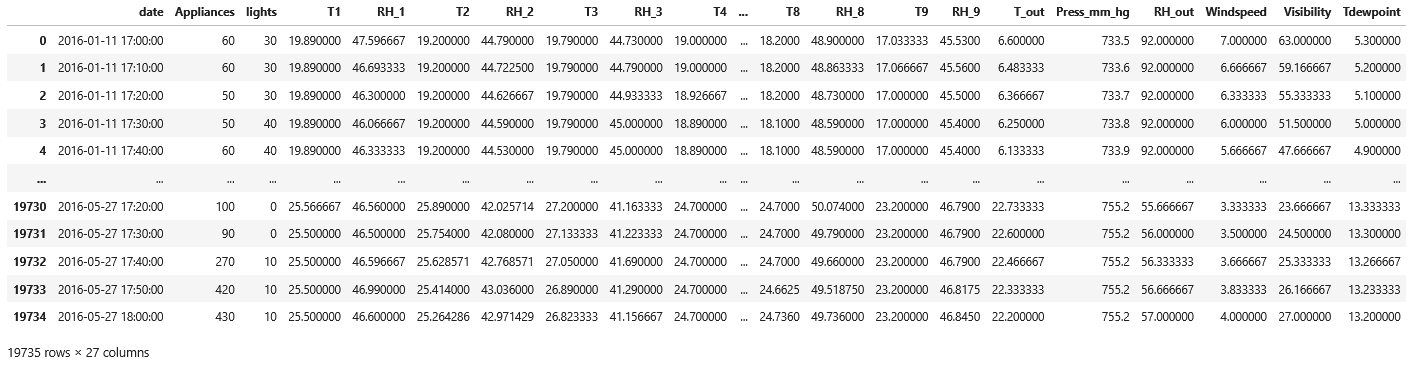
\includegraphics[width=\linewidth]{images/dataset.PNG}
    \caption{Tập dữ liệu \texttt{energydata\_complete.csv}}
\end{figure} 

Tập dữ liệu \texttt{energydata\_complete.csv} được sử dụng trong bài báo cáo này gồm các yếu tố ảnh hưởng đến mức tiêu thụ năng lượng trong toàn bộ ngôi nhà (đơn vị: Wh), cụ thể:
\begin{itemize}
    \item Dữ liệu cảm biến không dây: Nhiệt độ (\texttt{T1} đến \texttt{T9}, đơn vị: °C) và độ ẩm tương đối (\texttt{RH1} đến \texttt{RH9}, đơn vị: \%) được đo từ các cảm biến được trong các phòng khác nhau, lần lượt là bếp, phòng khách, phòng giặt, phòng làm việc, phòng tắm, phía Bắc bên ngoài tòa nhà, phòng ủi, phòng của con, phòng của cha mẹ.
    \item Dữ liệu thời tiết: Thu thập từ trạm thời tiết gần nhất, bao gồm các thông số như áp suất khí quyển (\texttt{Press\_mm\_hg}, đơn vị: mmHg), nhiệt độ ngoài trời (\texttt{T\_out}, đơn vị: °C), độ ẩm ngoài trời (\texttt{RH\_out}, đơn vị: \%), tốc độ gió (\texttt{Windspeed}, đơn vị: m/s), tầm nhìn (\texttt{Visibility}, đơn vị: km) và điểm sương (\texttt{Tdewpoint}, đơn vị: °C).
    \item Dữ liệu năng lượng: Mức tiêu thụ năng lượng của hệ thống chiếu sáng (\texttt{lights}, đơn vị: Wh).
    \item Thời gian thu thập: 137 ngày (4.5 tháng), với dữ liệu năng lượng được ghi lại mỗi 10 phút và dữ liệu thời tiết được nội suy từ khoảng thời gian 1 tiếng thành khoảng thời gian 10 phút.
    \item Số lượng mẫu và đặc trưng: Tập dữ liệu gồm có 19735 mẫu và 27 đặc trưng.
    \item Phân chia dữ liệu: Bộ dữ liệu được chia thành tập huấn luyện (75\% dữ liệu) dùng để xây dựng mô hình và tập kiểm tra (25\% dữ liệu) dùng để đánh giá mô hình.
\end{itemize}

\subsection{Phân tích dữ liệu}
Hai hình dưới đây minh hoạ mức tiêu thụ năng lượng trong khoảng thời gian 137 ngày (4.5 tháng) và trong tuần đầu tiên của tập dữ liệu. Chúng ta có thể quan sát thấy mức tiêu thụ năng lượng có sự biến động cao.
\begin{figure}[H]
    \centering
    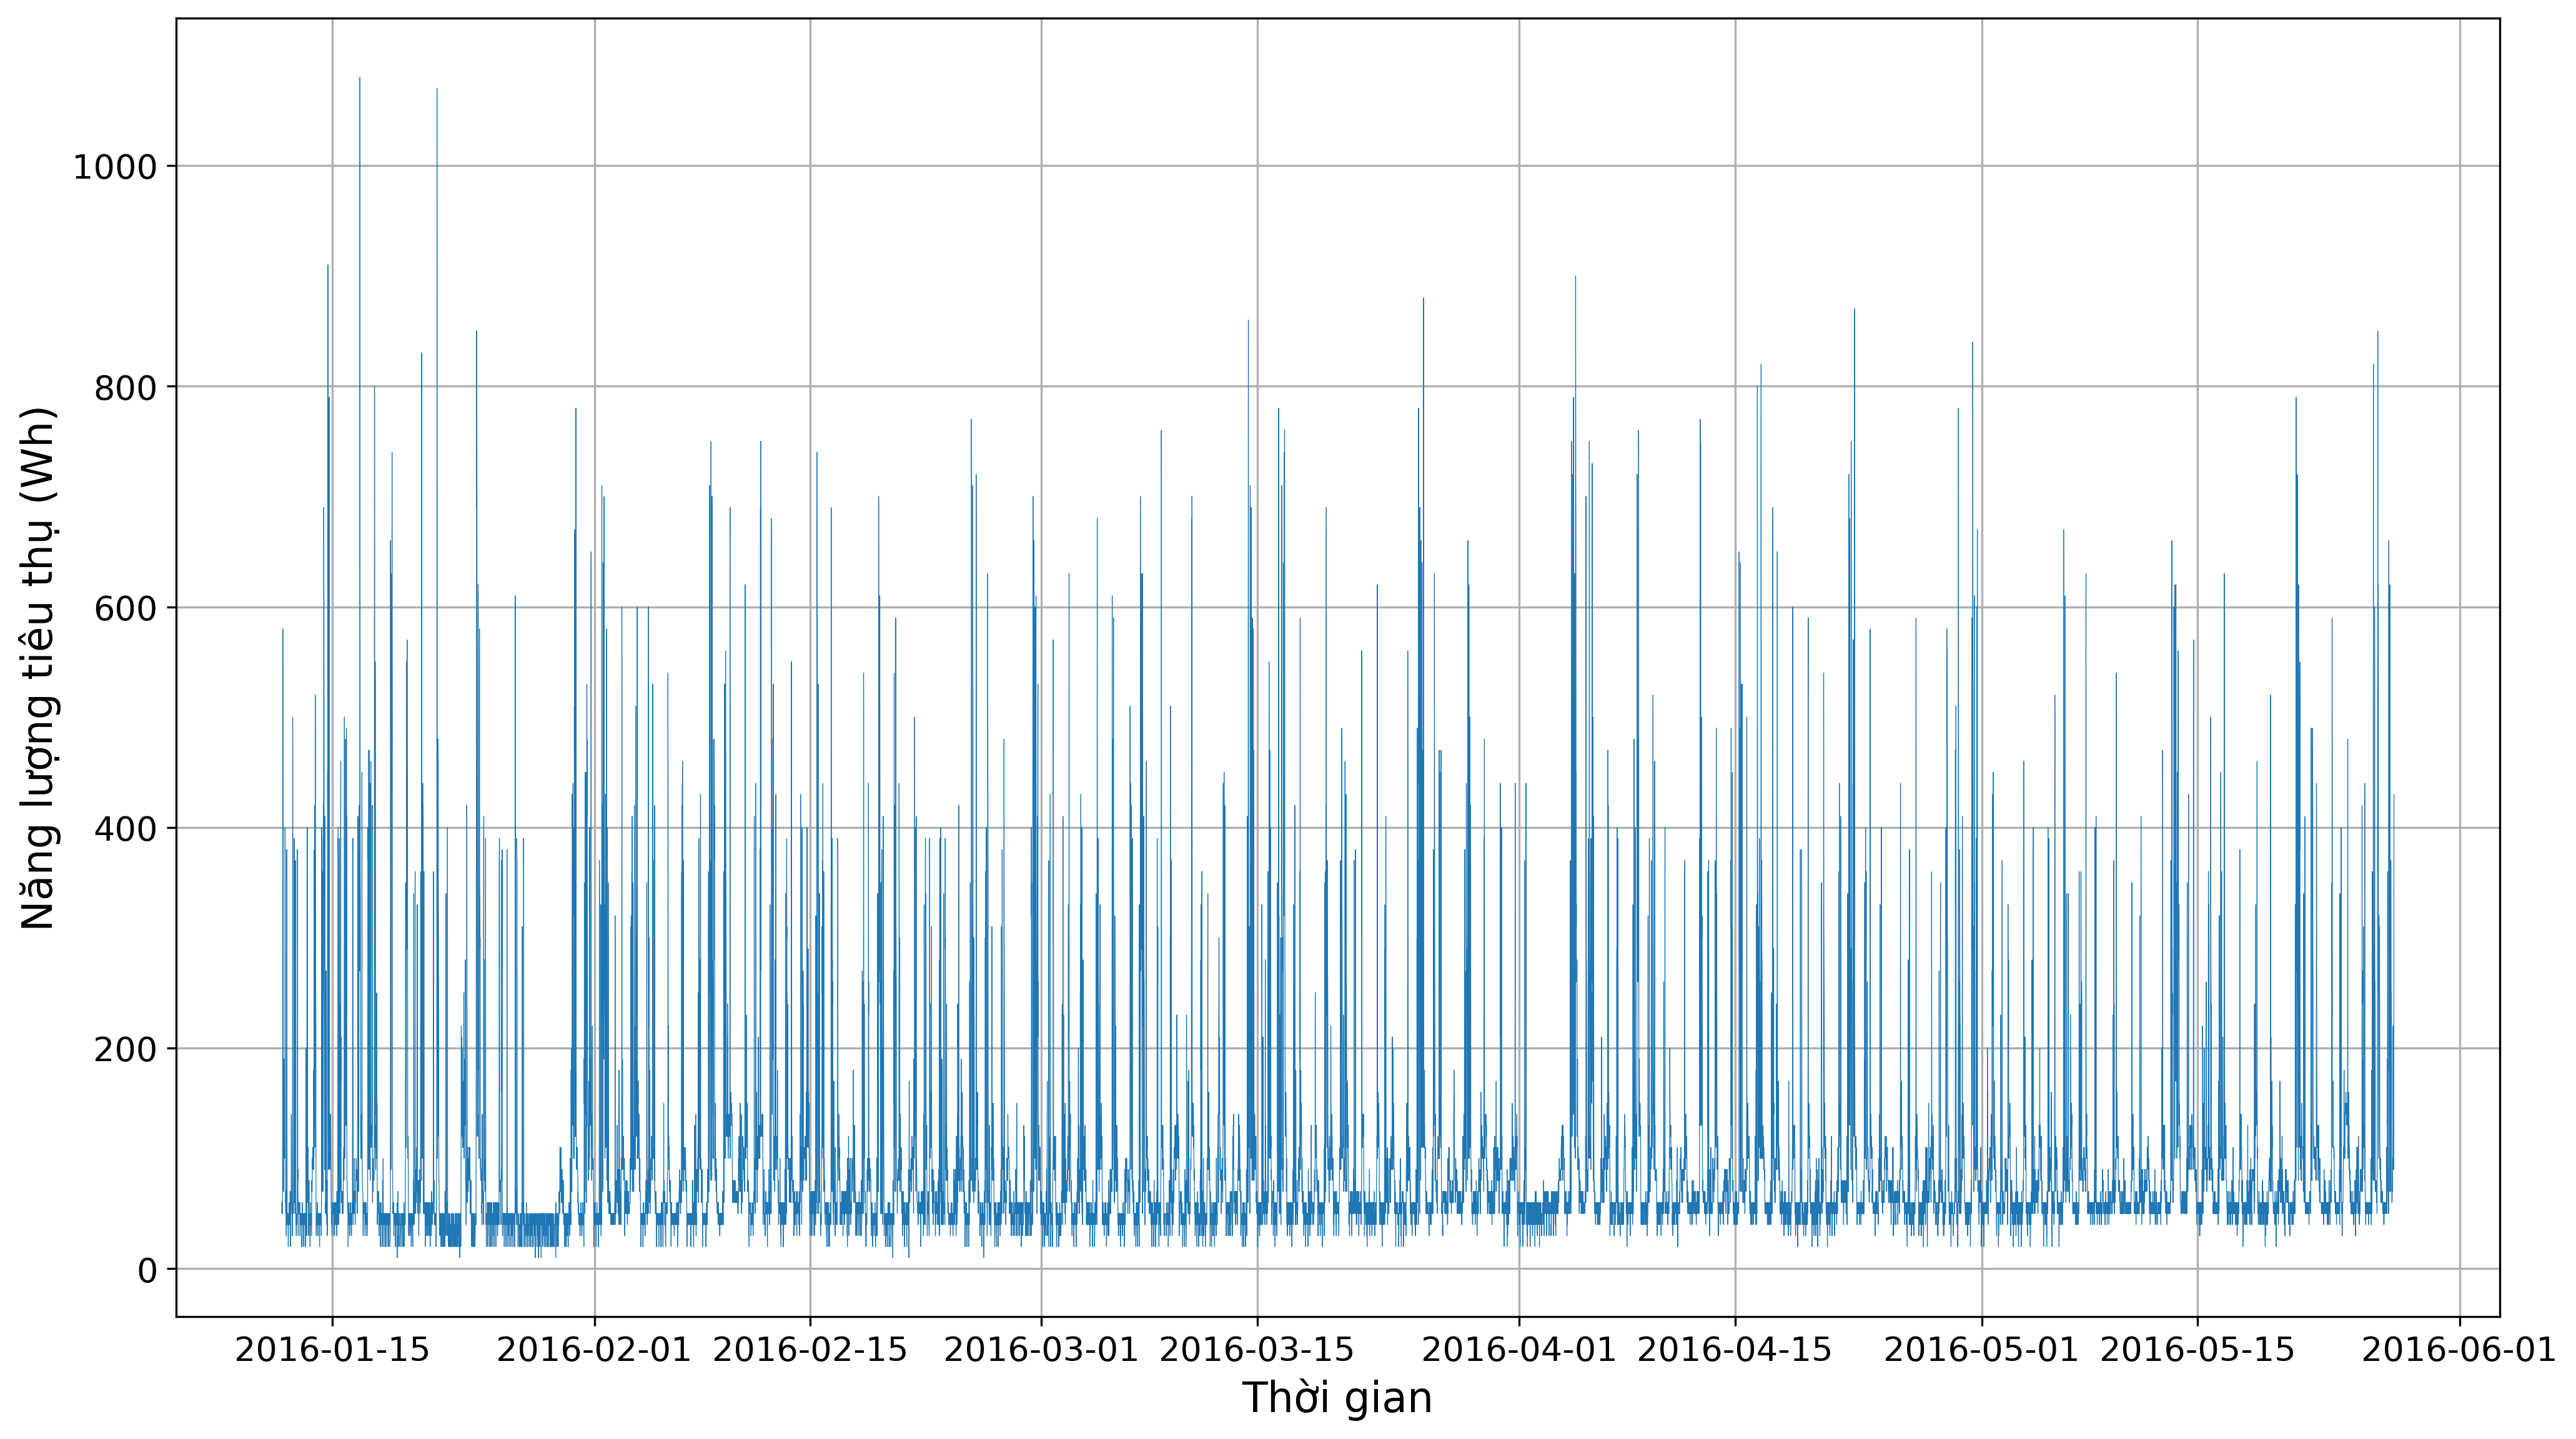
\includegraphics[width=\linewidth]{images/energy_consumption_137days.png}
    \caption{Mức tiêu thụ năng lượng trong toàn bộ tập dữ liệu (137 ngày)}
\end{figure} 
\begin{figure}[H]
    \centering
    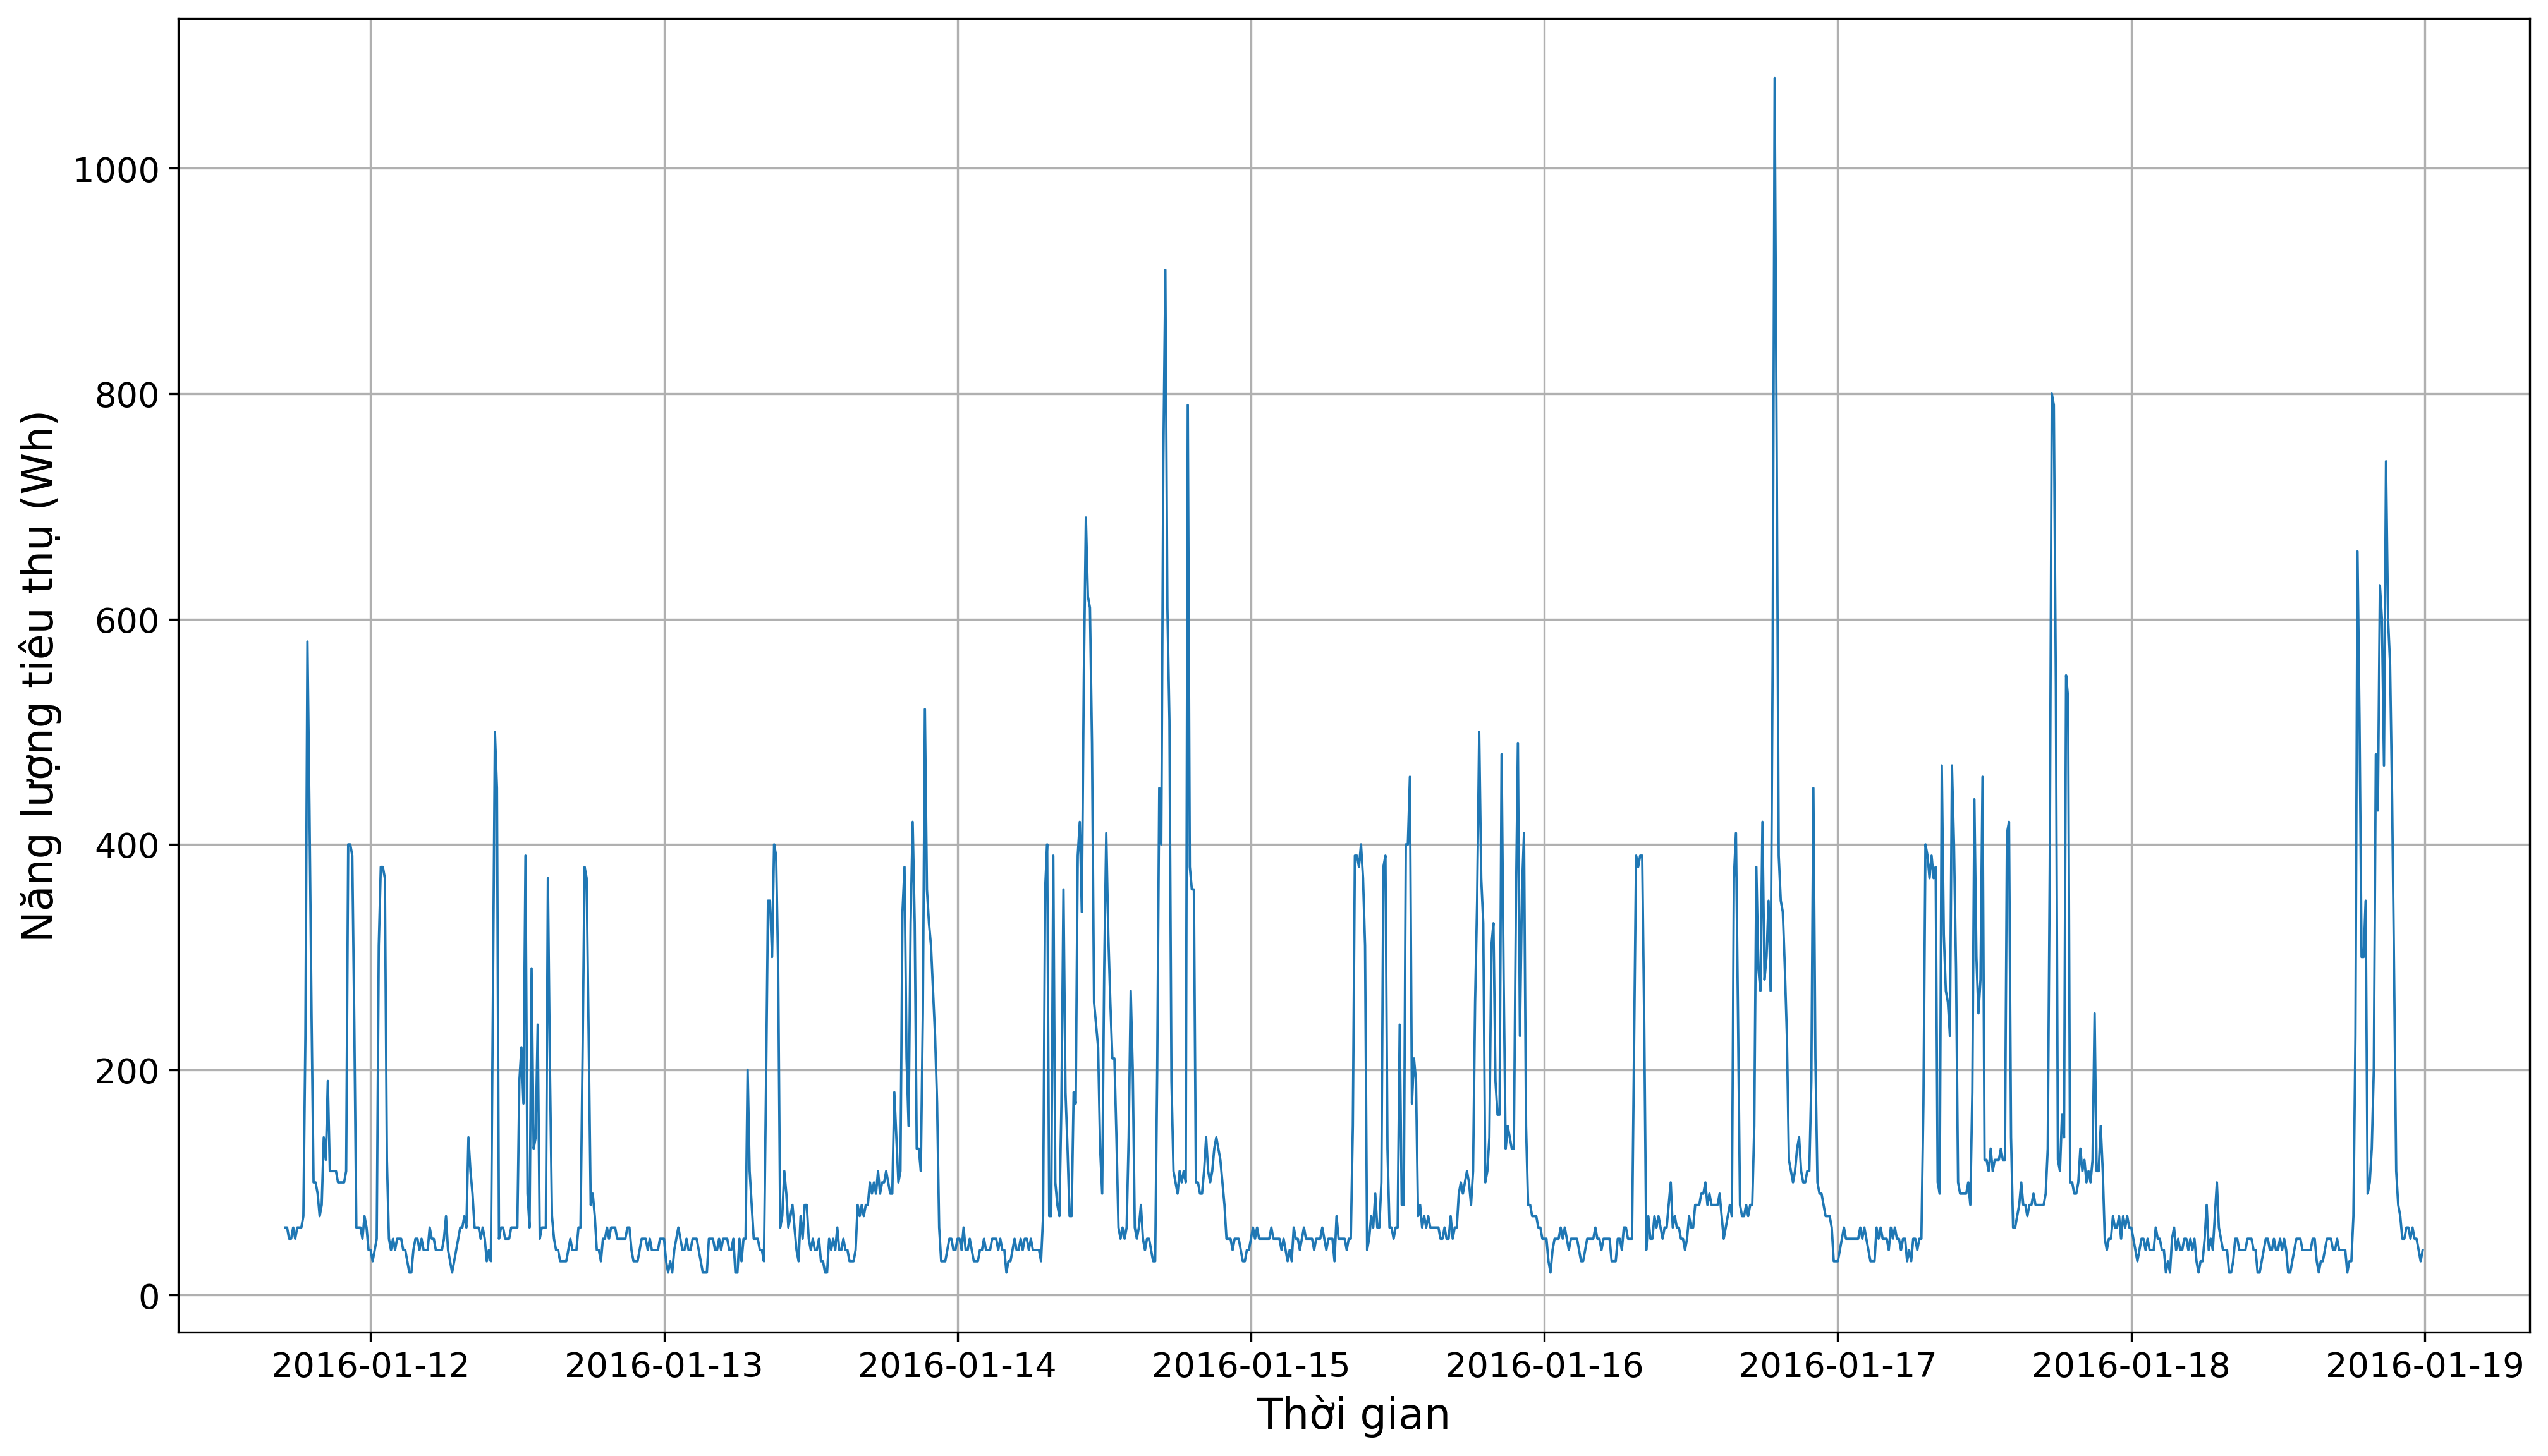
\includegraphics[width=\linewidth]{images/energy_consumption_first7days.png}
    \caption{Mức tiêu thụ năng lượng trong 1 tuần đầu tiên của tập dữ liệu}
\end{figure}

Hai hình tiếp theo trình bày biểu đồ histogram và boxplot của tập dữ liệu. Biểu đồ histogram thể hiện tần suất phân phối của các giá trị, trong khi boxplot cho thấy được các đặc trưng thống kê như trung vị, tứ phân vị và các giá trị ngoại lai. Hai biểu đồ này giúp đánh giá trực quan mức độ phân tán và xu hướng của tập dữ liệu.
\begin{figure}[H]
    \centering
    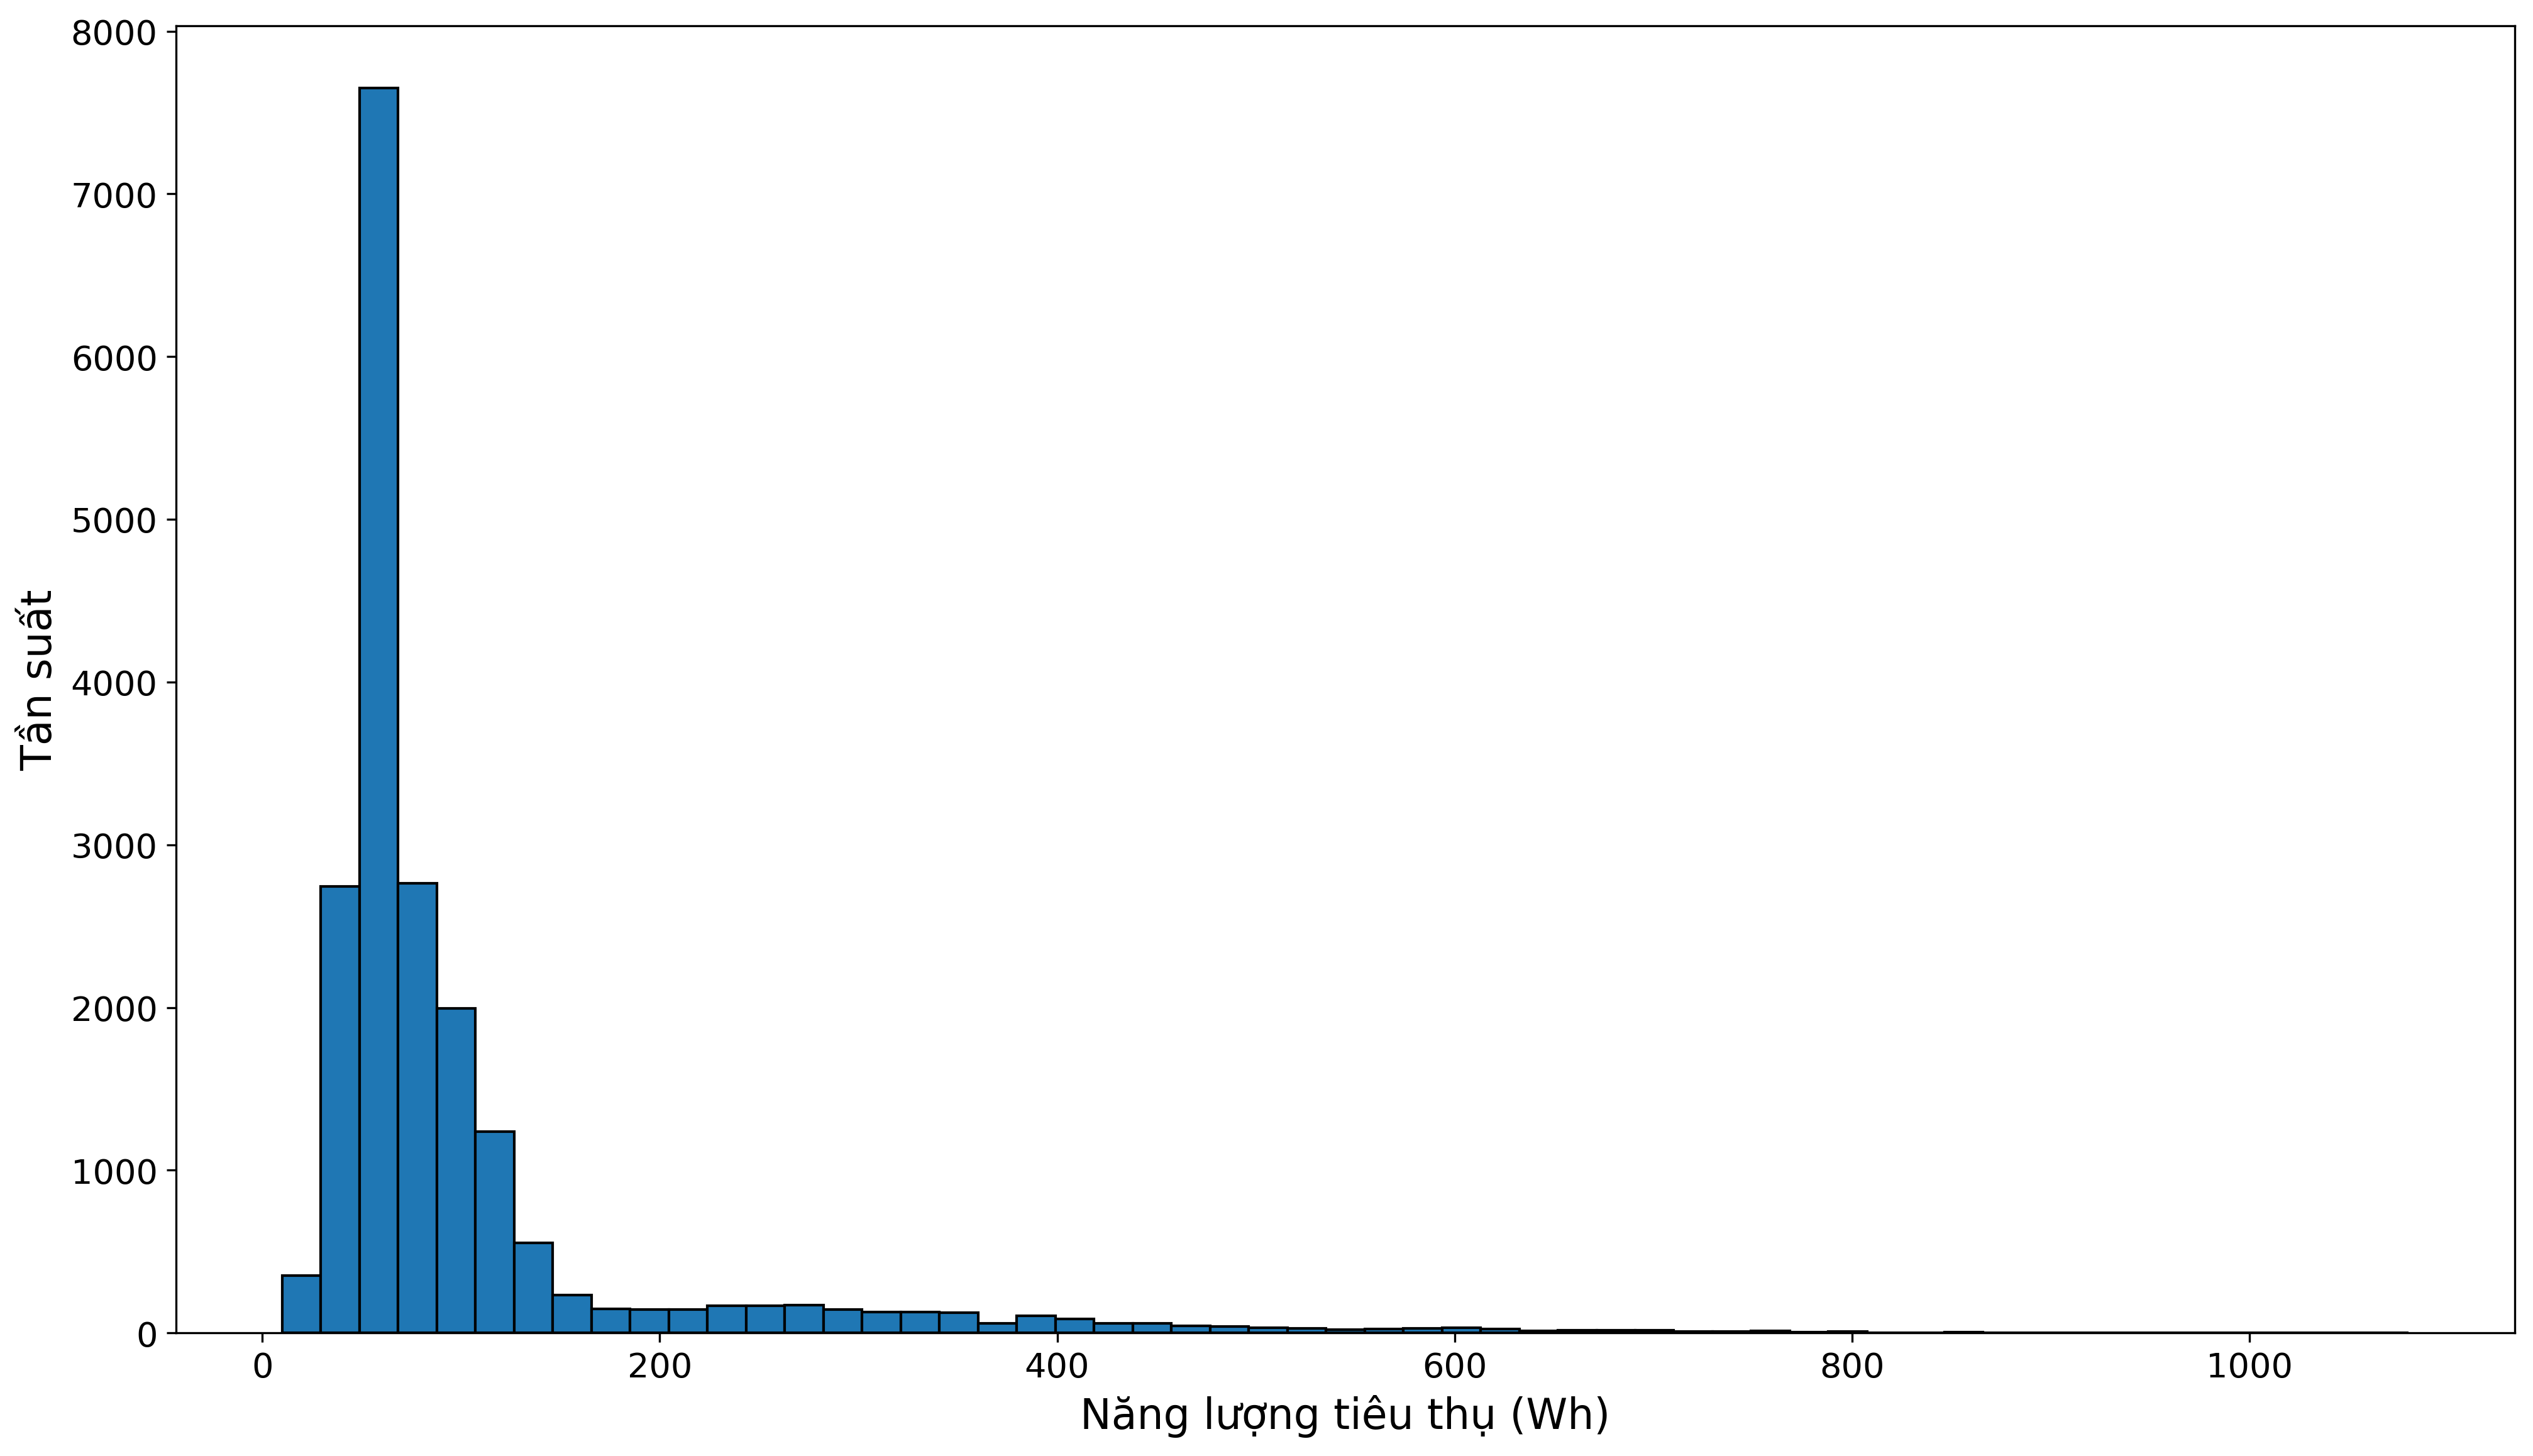
\includegraphics[width=\linewidth]{images/histogram.png}
    \caption{Biểu đồ histogram của tập dữ liệu}
\end{figure}
\begin{figure}[H]
    \centering
    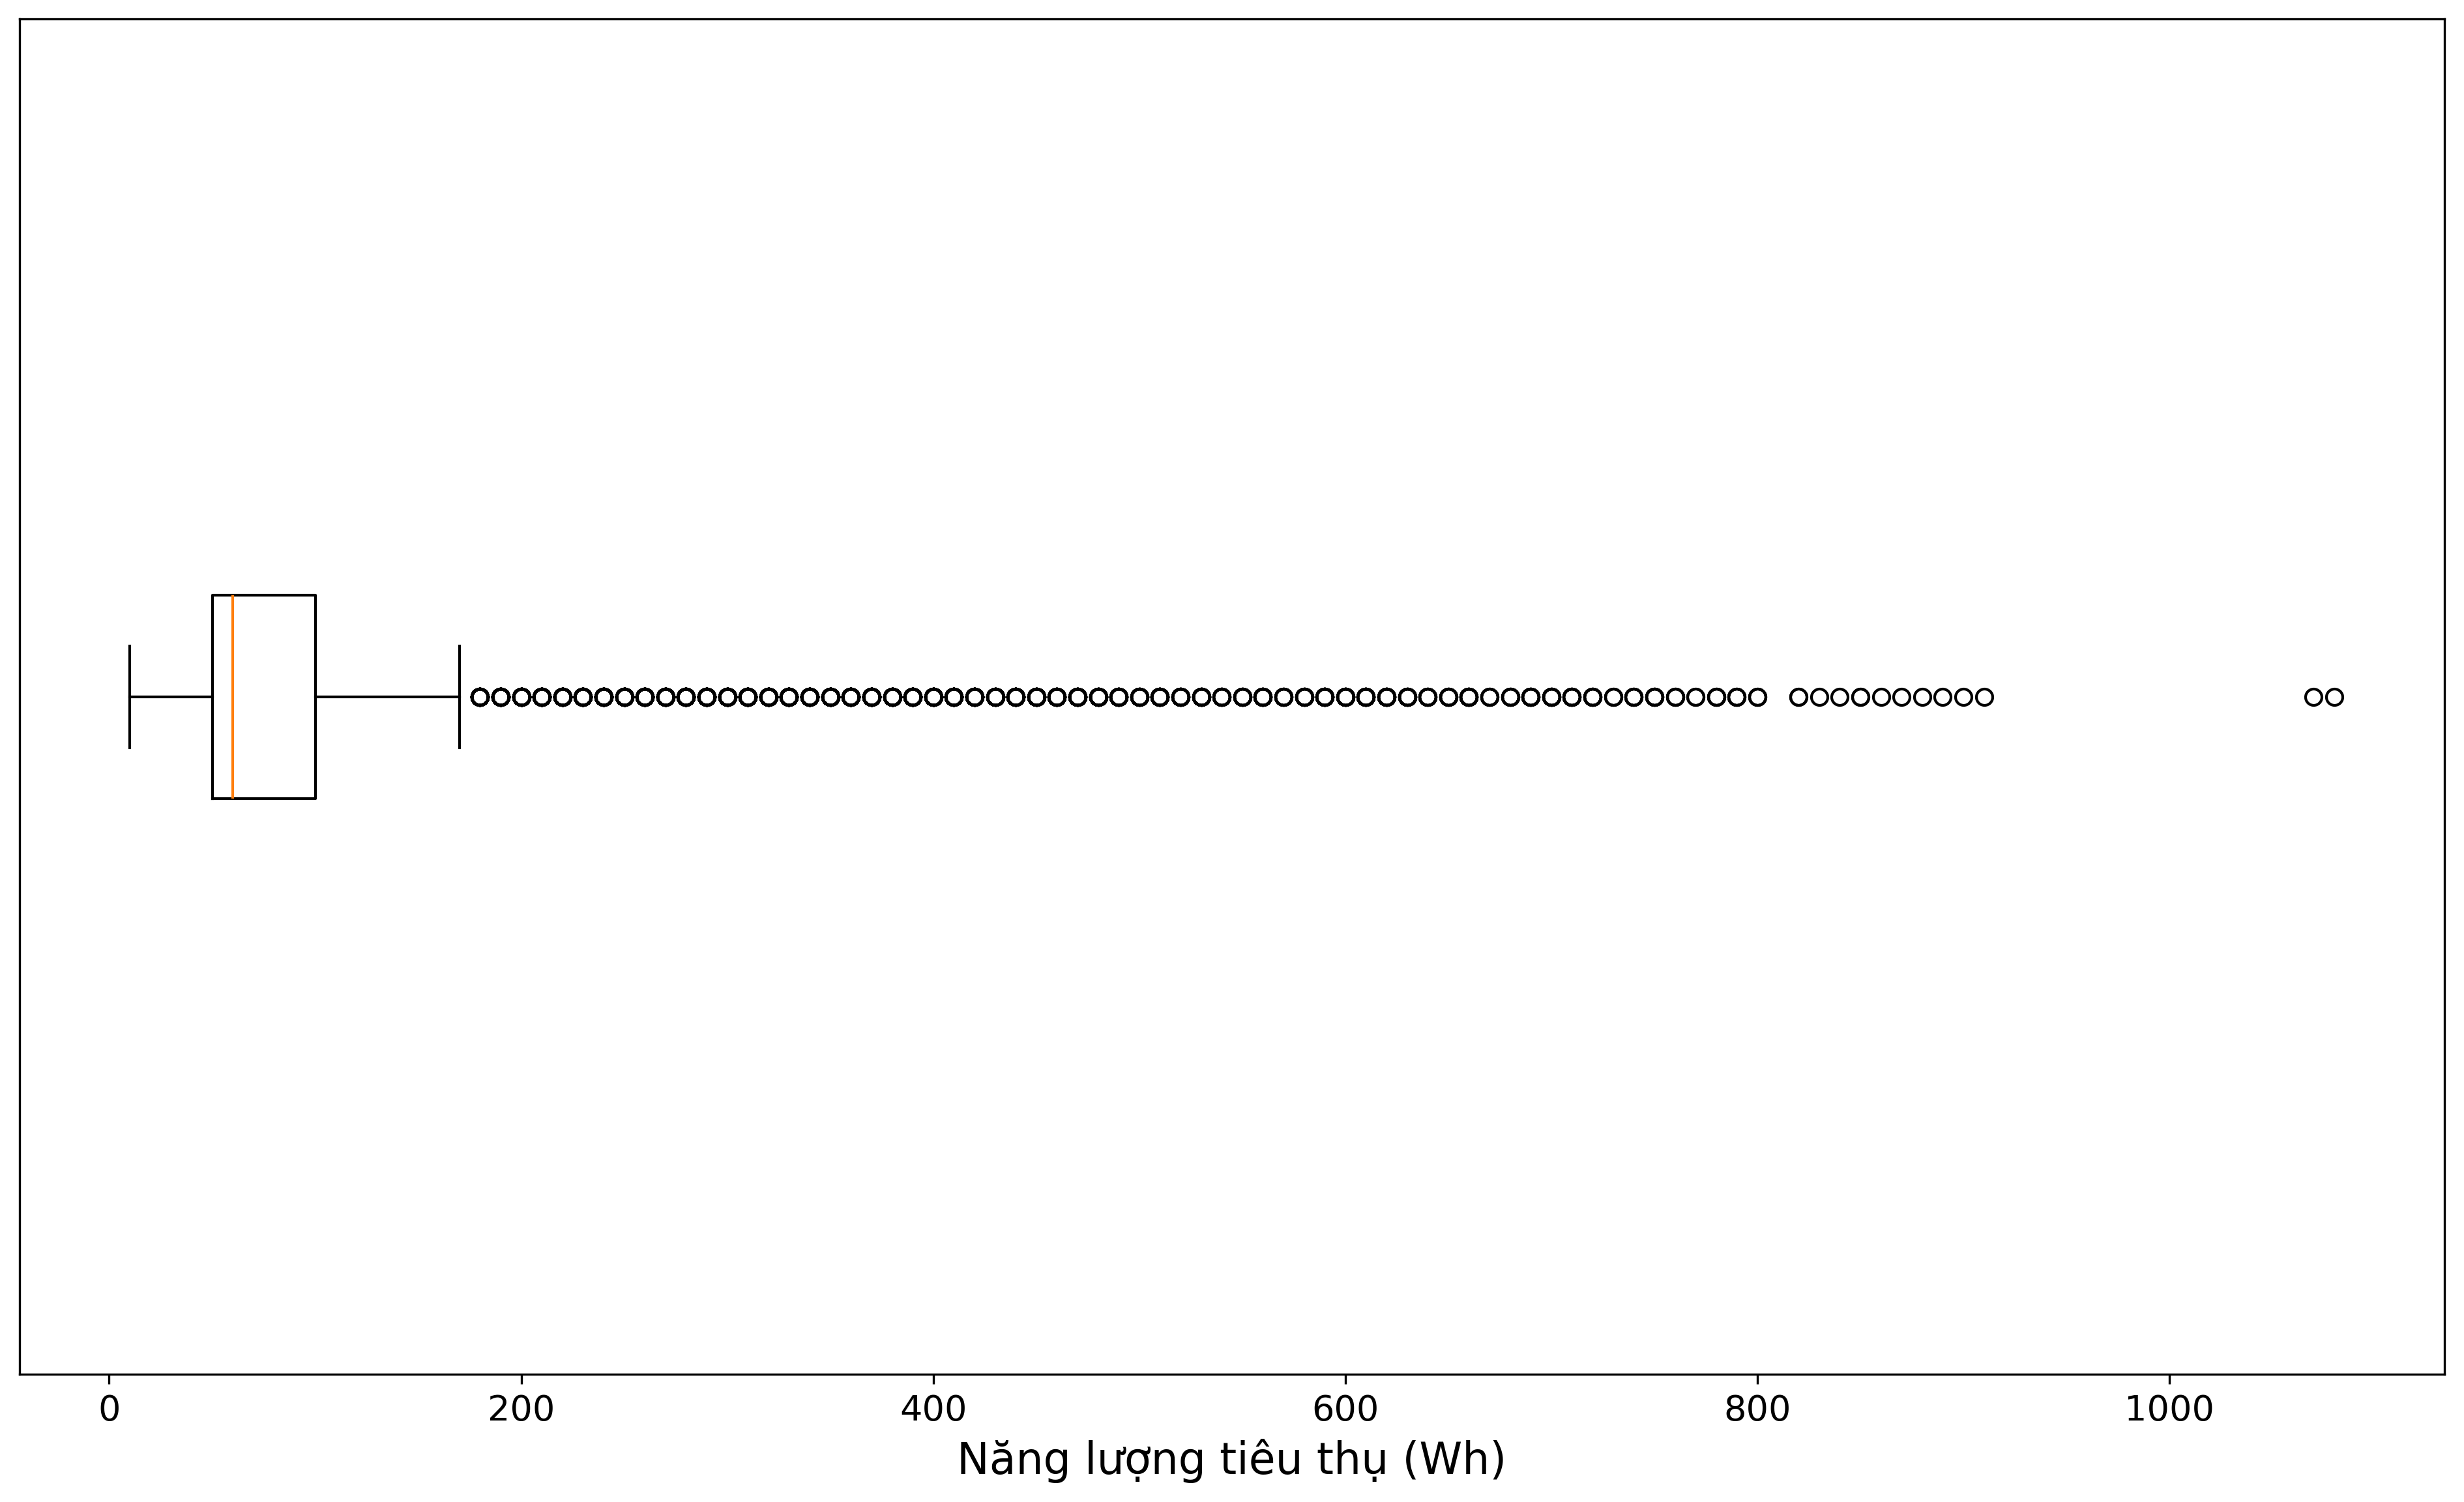
\includegraphics[width=\linewidth]{images/boxplot.png}
    \caption{Biểu đồ boxplot của tập dữ liệu}
\end{figure}
Trong Hình 5, giá trị trung vị là 60 Wh, được thể hiện bằng đường màu cam trong hình chữ nhật, giới hạn dưới là 10 Wh và giới hạn trên là 170 Wh. Các giá trị phía trên trung vị có độ phân tán lớn hơn, với nhiều điểm ngoại lai được đánh dấu bằng các vòng tròn phía trên giới hạn trên.

Dữ liệu cho thấy được mức sử dụng năng lượng trong nhà có sự biến động lớn, trung vị 60 Wh nhưng có nhiều giá trị ngoại lai, cho thấy sự đa dạng trong thói quen sử dụng, cũng như có vai trò quan trọng trong việc phân tích các yếu tố ảnh hưởng đến mức tiêu thụ năng lượng, từ đó hỗ trợ xây dựng các mô hình dự đoán chính xác hơn.

\newpage
\subsection{Lựa chọn mô hình}
Để dự đoán được mức tiêu thụ năng lượng của các thiết bị dựa vào dữ liệu lịch sử, có 3 mô hình dự đoán được chọn để so sánh dựa trên tính phổ biến trong các bài toán hồi quy:
\subsubsection{Multiple Linear Regression}
Multiple Linear Regression là một phương pháp thống kê nhằm mô hình hoá mối quan hệ tuyến giữa một biến phụ thuộc (ở đây là mức tiêu thụ năng lượng) và nhiều biến độc lập (các đặc trưng như nhiệt độ, độ ẩm,...). Mô hình giả định rằng biến phụ thuộc có thể được biểu diễn dưới dạng một tổ hợp tuyến tính của các biến độc lập:
\[\hat{y} = \theta_0 + \theta_1x_1 + \theta_2x_2 + ... + \theta_nx_n\]
trong đó \(y\) là biến phụ thuộc, \(x_i\), \(\theta_i\) là các hệ số hồi quy.

\begin{figure}[H]
    \centering
    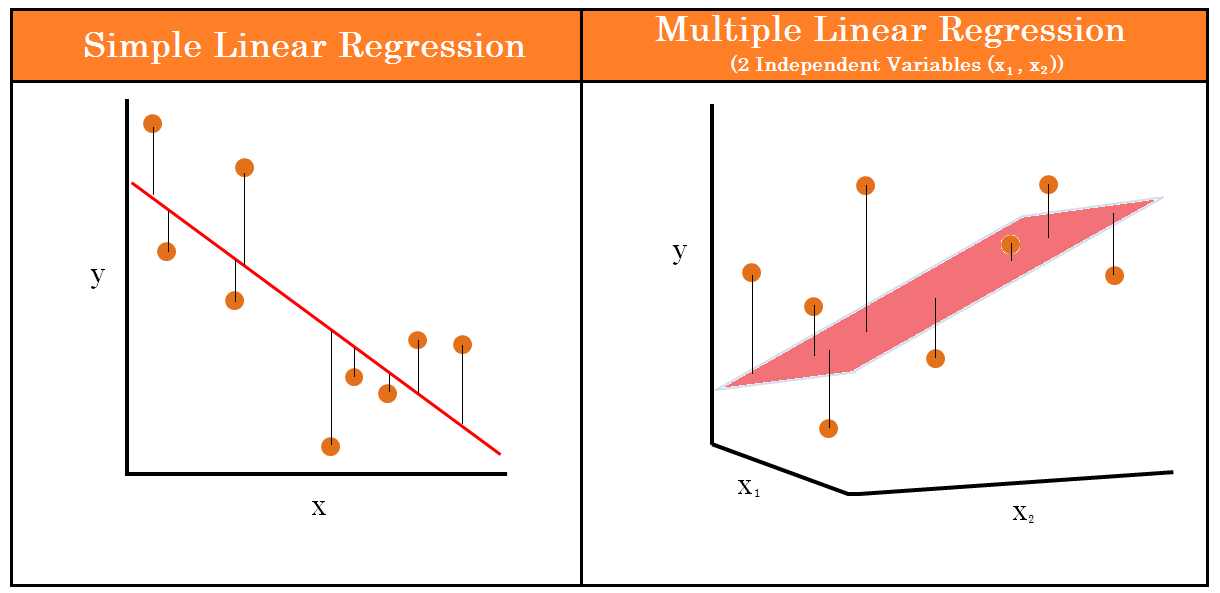
\includegraphics[width=\linewidth]{images/LR.png}
    \caption{Linear Regression và Multiple Linear Regression}
\end{figure}

Multiple Linear Regression được chọn vì tính đơn giản và khả năng diễn giải trực quan, giúp xác định mức độ ảnh hưởng của từng yếu tố đến mức tiêu thụ năng lượng. Cũng như có thể dùng làm mô hình cơ sở để so sánh hiệu suất với các mô hình phức tạp hơn như Random Forest hoặc Gradient Boosting Machine. Tuy nhiên, mô hình này bị hạn chế trong việc xử lý các mối quan hệ phi tuyến hoặc dữ liệu phức tạp, dễ bị ảnh hưởng bởi giá trị ngoại lai.

\newpage
\subsubsection{Random Forest}
Random Forest là một mô hình dự đoán dựa trên phương pháp tập hợp mô hình (ensemble-based method). Mô hình này giúp giảm thiểu phương sai bằng cách kết hợp kết quả từ nhiều Decision Tree, từ đó hạn chế hiện tượng quá khớp so với việc một Decision Tree đơn lẻ. Mỗi Decision Tree được huấn luyện trên một tập con ngẫu nhiên của dữ liệu (bootstrap sampling). Dự đoán cuối cùng được tính bằng trung bình các dự đoán từ tất cả các Decision Tree:
\[\hat{y} = \frac{1}{T}\sum_{t=1}^{T}{y_t(x)}\]
trong đó \(T\) là số cây, \(y_t(x)\) là dự đoán của cây thứ \(t\).

\begin{figure}[H]
    \centering
    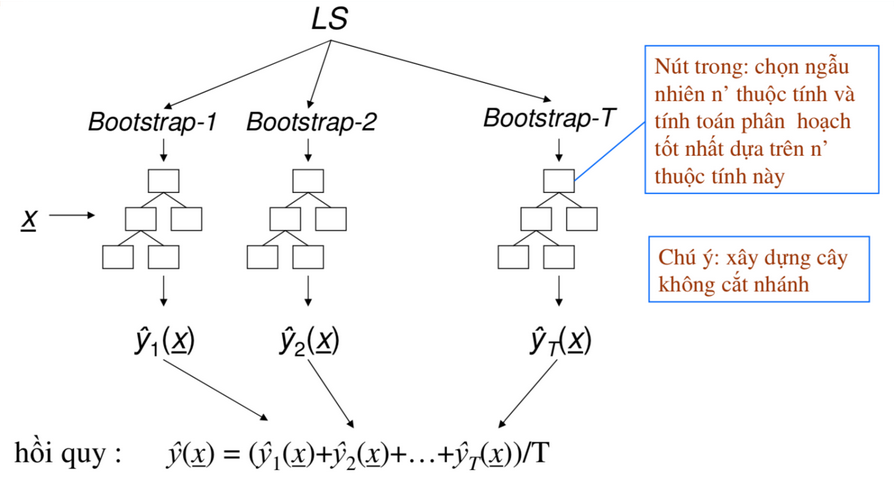
\includegraphics[width=\linewidth]{images/RF.png}
    \caption{Random Forest}
\end{figure}

Random Forest được chọn vì khả năng nắm bắt các mối quan hệ phi tuyến phức tạp giữa các đặc trưng và mức tiêu thụ năng lượng, cũng như là có thể cung cấp được bảng xếp hạng tầm quan trọng của các đặc trưng, hữu ích trong việc xác định các yếu tố ảnh hưởng chính. Ngoài ra, mô hình này có độ ổn định cao và ít nhạy cảm với giá trị ngoại lai, phù hợp với bộ dữ liệu có biến động lớn. Tuy nhiên, mô hình yêu cầu phải phần cứng đủ tốt để đáp ứng được việc tính toán số lượng lớn Decision Tree.

\newpage
\subsubsection{Gradient Boosting Machine}
Gradient Boosting Machine là một mô hình dự đoán dựa trên phương pháp tập hợp mô hình (ensemble-based method). Mô hình này giúp giảm thiểu sai số bằng cách kết hợp tuần tự các Decision Tree, trong đó mỗi Decision Tree mới được huấn luyện để sửa lỗi (residual) còn sót lại của các Decision Tree trước đó bằng cách sử dụng phương pháp tối ưu hóa hàm mất mát (loss function) thông qua kĩ thuật gradient descent, từ đó nâng cao độ chính xác so với một cây đơn lẻ. Dự đoán cuối cùng được tính bằng tổng có trọng số của tất cả các cây trong chuỗi:
\[Y_t(x) = Y_{t-1}(x) + \eta y_t(x)\]
trong đó, \(Y_t(x)\) là mô hình tại bước \(t\), \(y_t(x)\) là dự đoán của cây thứ \(t\), và \(\eta\) là tốc độ học.

\begin{figure}[H]
    \centering
    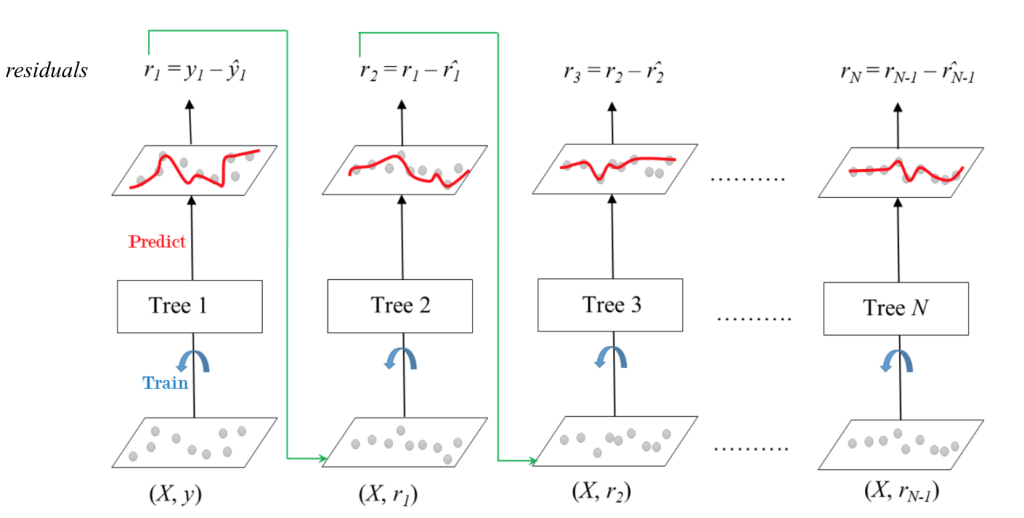
\includegraphics[width=\linewidth]{images/GBM.png}
    \caption{Gradient Boosting Machine}
\end{figure}

Gradient Boosting Machine được chọn vì khả năng vượt trội trong việc xử lý dữ liệu phức tạp, có khả năng xử lý các mối quan hệ phi tuyến và tương tác giữa các đặc trưng, cũng nhưng là có thể cung cấp thông tin về tầm quan trọng của các đặc trưng, giúp xác định các yếu tố then chốt. Tuy nhiên, mô hình rất dễ bị quá khớp nếu không điều chỉnh tham số cẩn thận, và tốn nhiều thời gian tính toán hơn so với Random Forest.

\subsection{Cấu hình máy tính}
\begin{figure}[H]
    \centering
    
\includegraphics[width=\linewidth]{images/computer.PNG}
    \caption{Cấu hình máy tính dùng để huấn luyện mô hình}
\end{figure}
Quá trình huấn luyện sử dụng máy tính có cấu hình 16 GB RAM, vi xử lý AMD Ryzen 5 3600 6-Core 3.59 GHz, card đồ họa NVDIA GeForce RTX 2060 SUPER 8 GB, và hệ điều hành Kali Linux.

\subsection{Huấn luyện mô hình}
Để đảm bảo độ tin cậy của kết quả đánh giá hiệu suất ban đầu trước khi đánh giá mô hình trên tập kiểm tra, tất cả các mô hình đều được huấn luyện bằng phương pháp kiểm định chéo 10-fold (10-fold cross-validation) với 3 lần lặp trên tập huấn luyện.

\subsubsection{Multiple Linear Regression}
Multiple Linear Regression là mô hình đầu tiên được huấn luyện. Mô hình này sử dụng tất cả các biến dự đoán có sẵn để tìm ra các hệ số hồi quy, qua đó định lượng mức độ ảnh hưởng của từng biến đến mức tiêu thụ năng lượng.

Hình 10 cung cấp biểu đồ phần dư của mô hình Multiple Linear Regression, trong đó phần dư được tính bằng hiệu giữa giá trị thức tế và giá trị dự đoán:
\[\text{residual} = y - \hat{y}\]
Kết quả cho thấy phần dư không phân bố quanh trục hoành, điều này chỉ ra rằng mối quan hệ giữa các biến dự đoán và mức tiêu thụ năng lượng không mang tính tuyến tính. Do đó, mô hình Multiple Linear Regression không thể biểu diễn tốt dữ liệu trong trường hợp này.

\begin{figure}[H]
    \centering
    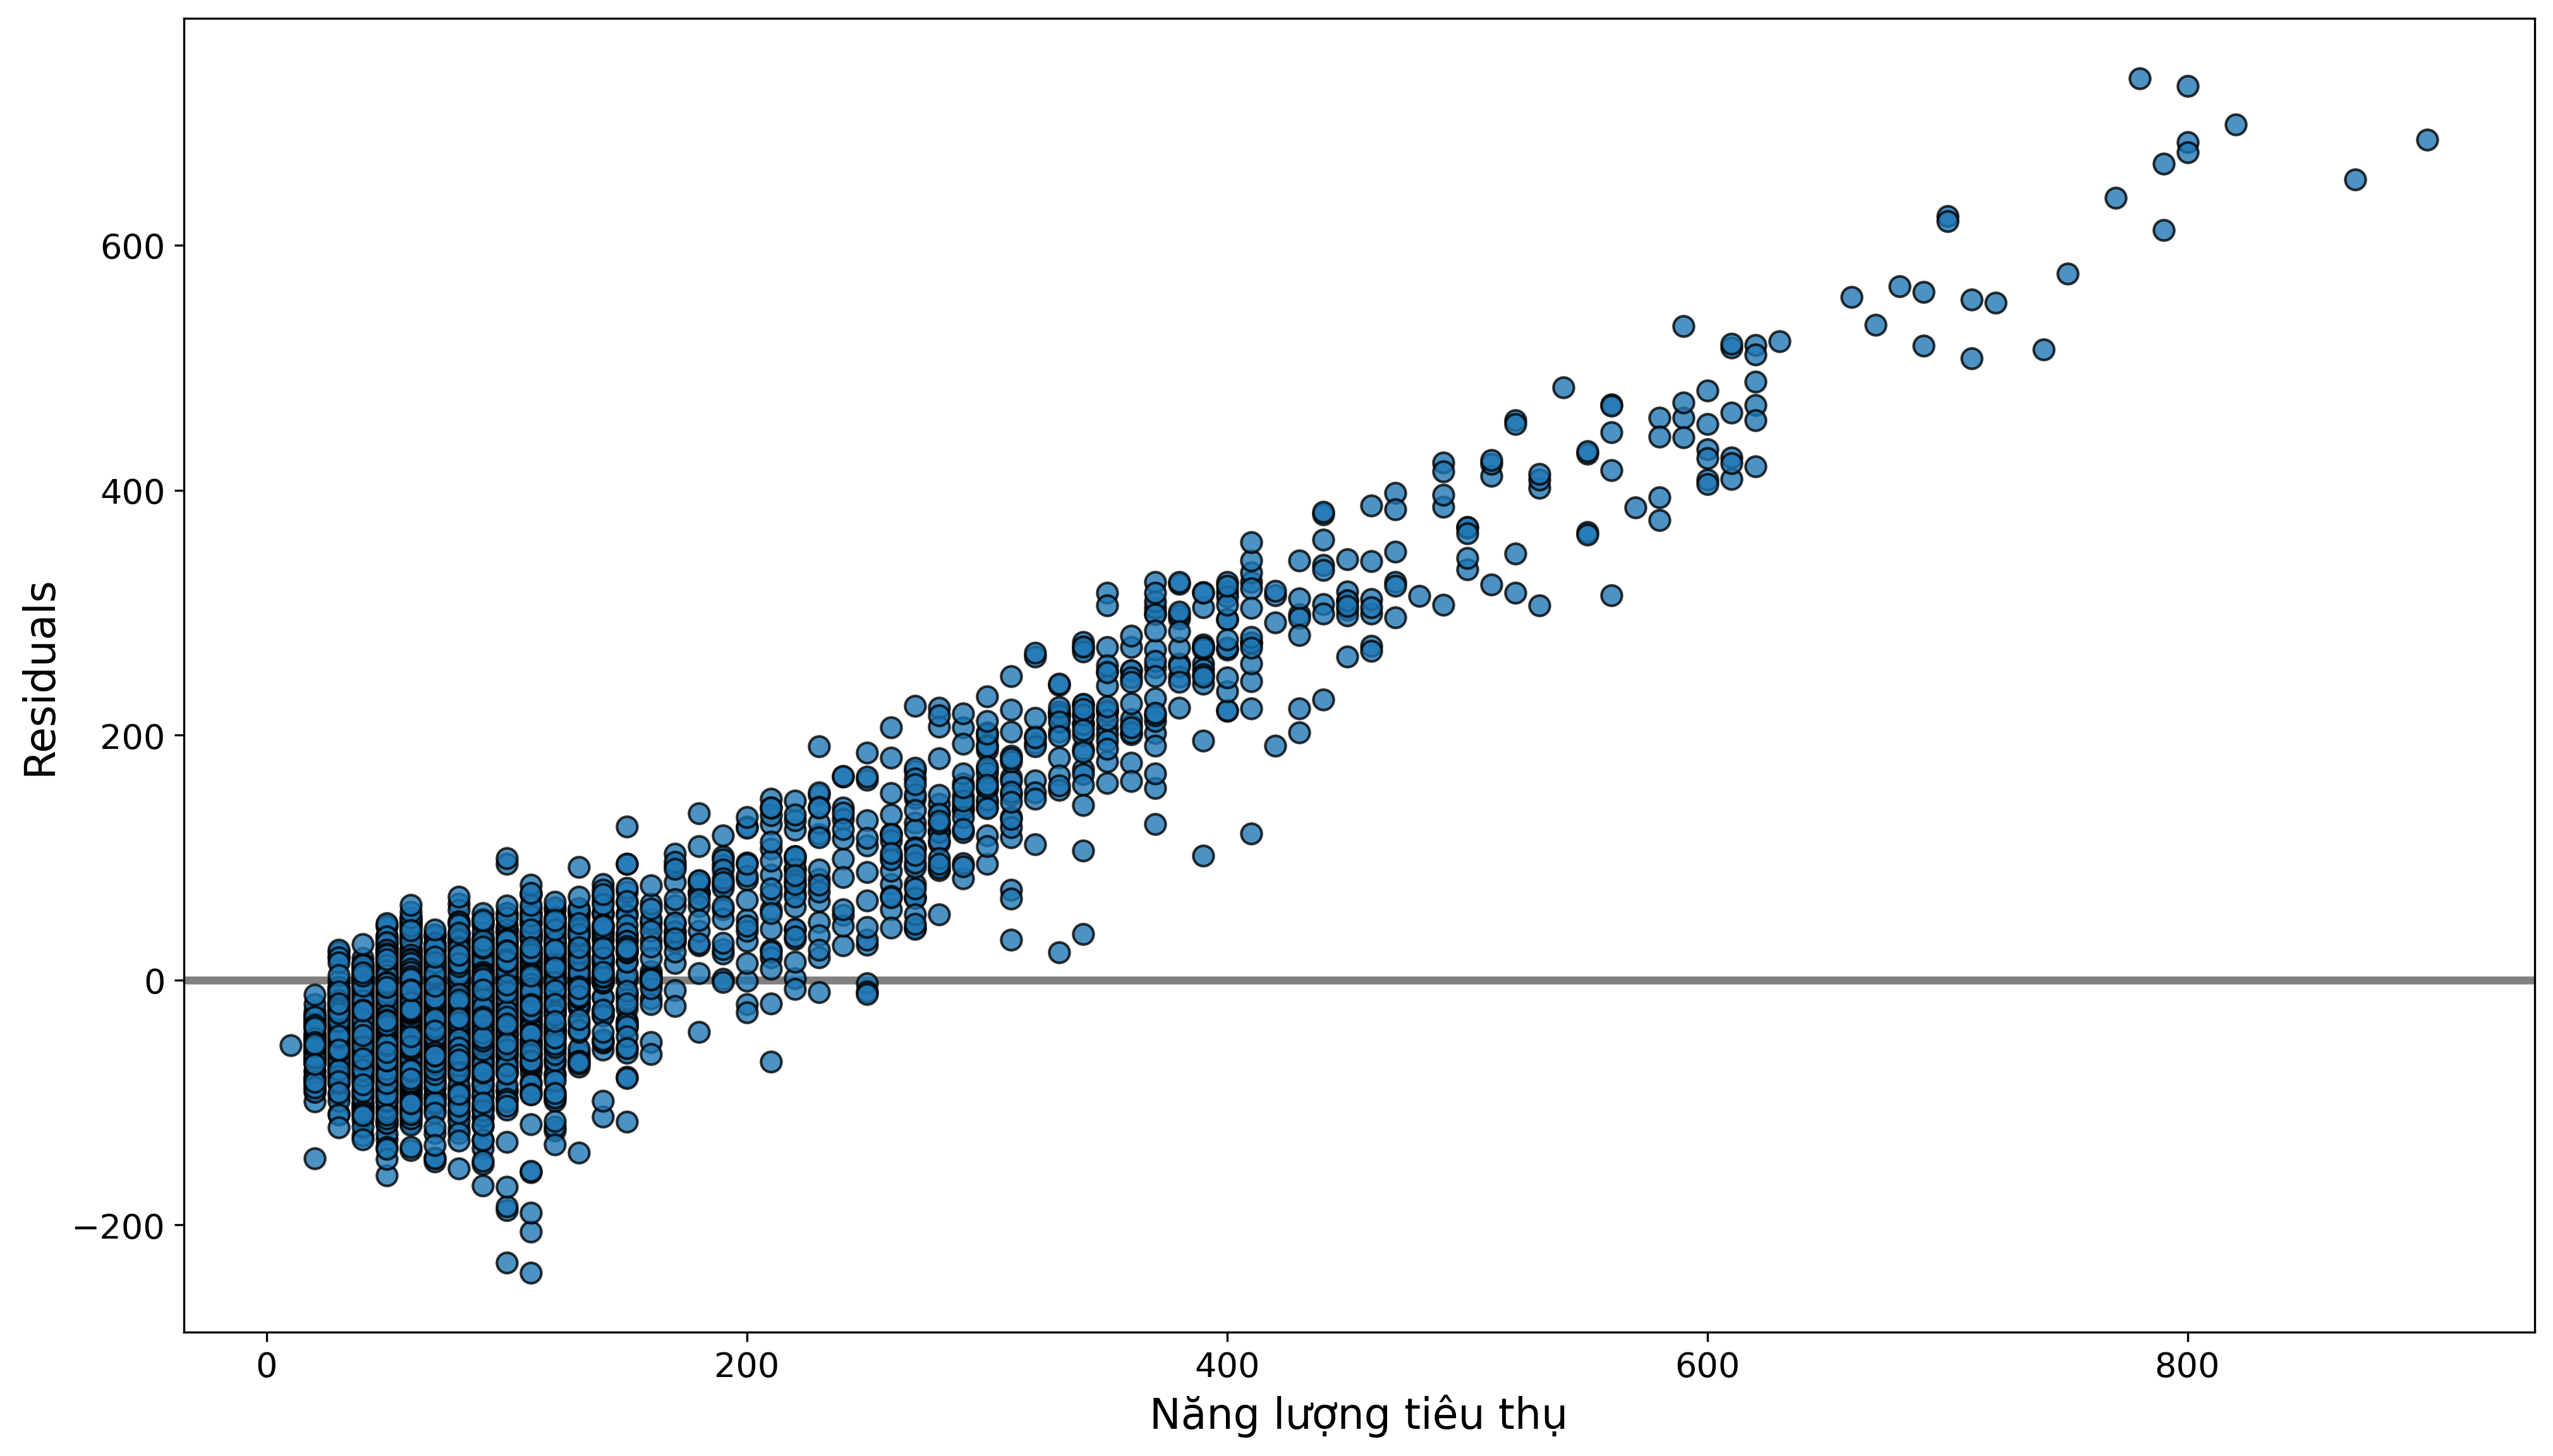
\includegraphics[width=\linewidth]{images/LR_residuals.png}
    \caption{Biểu đồ phần dư của mô hình Multiple Linear Regression}
\end{figure}

\subsubsection{Random Forest}
Random Forest là một mô hình dựa trên tập hợp dự đoán của nhiều Decision Trees, để tối ưu hóa mô hình, cần xác định số lượng Decision Tree của mô hình. Theo kết quả từ Hình 11, RMSE của mô hình ổn định sau khoảng 300 cây.
\begin{figure}[H]
    \centering
    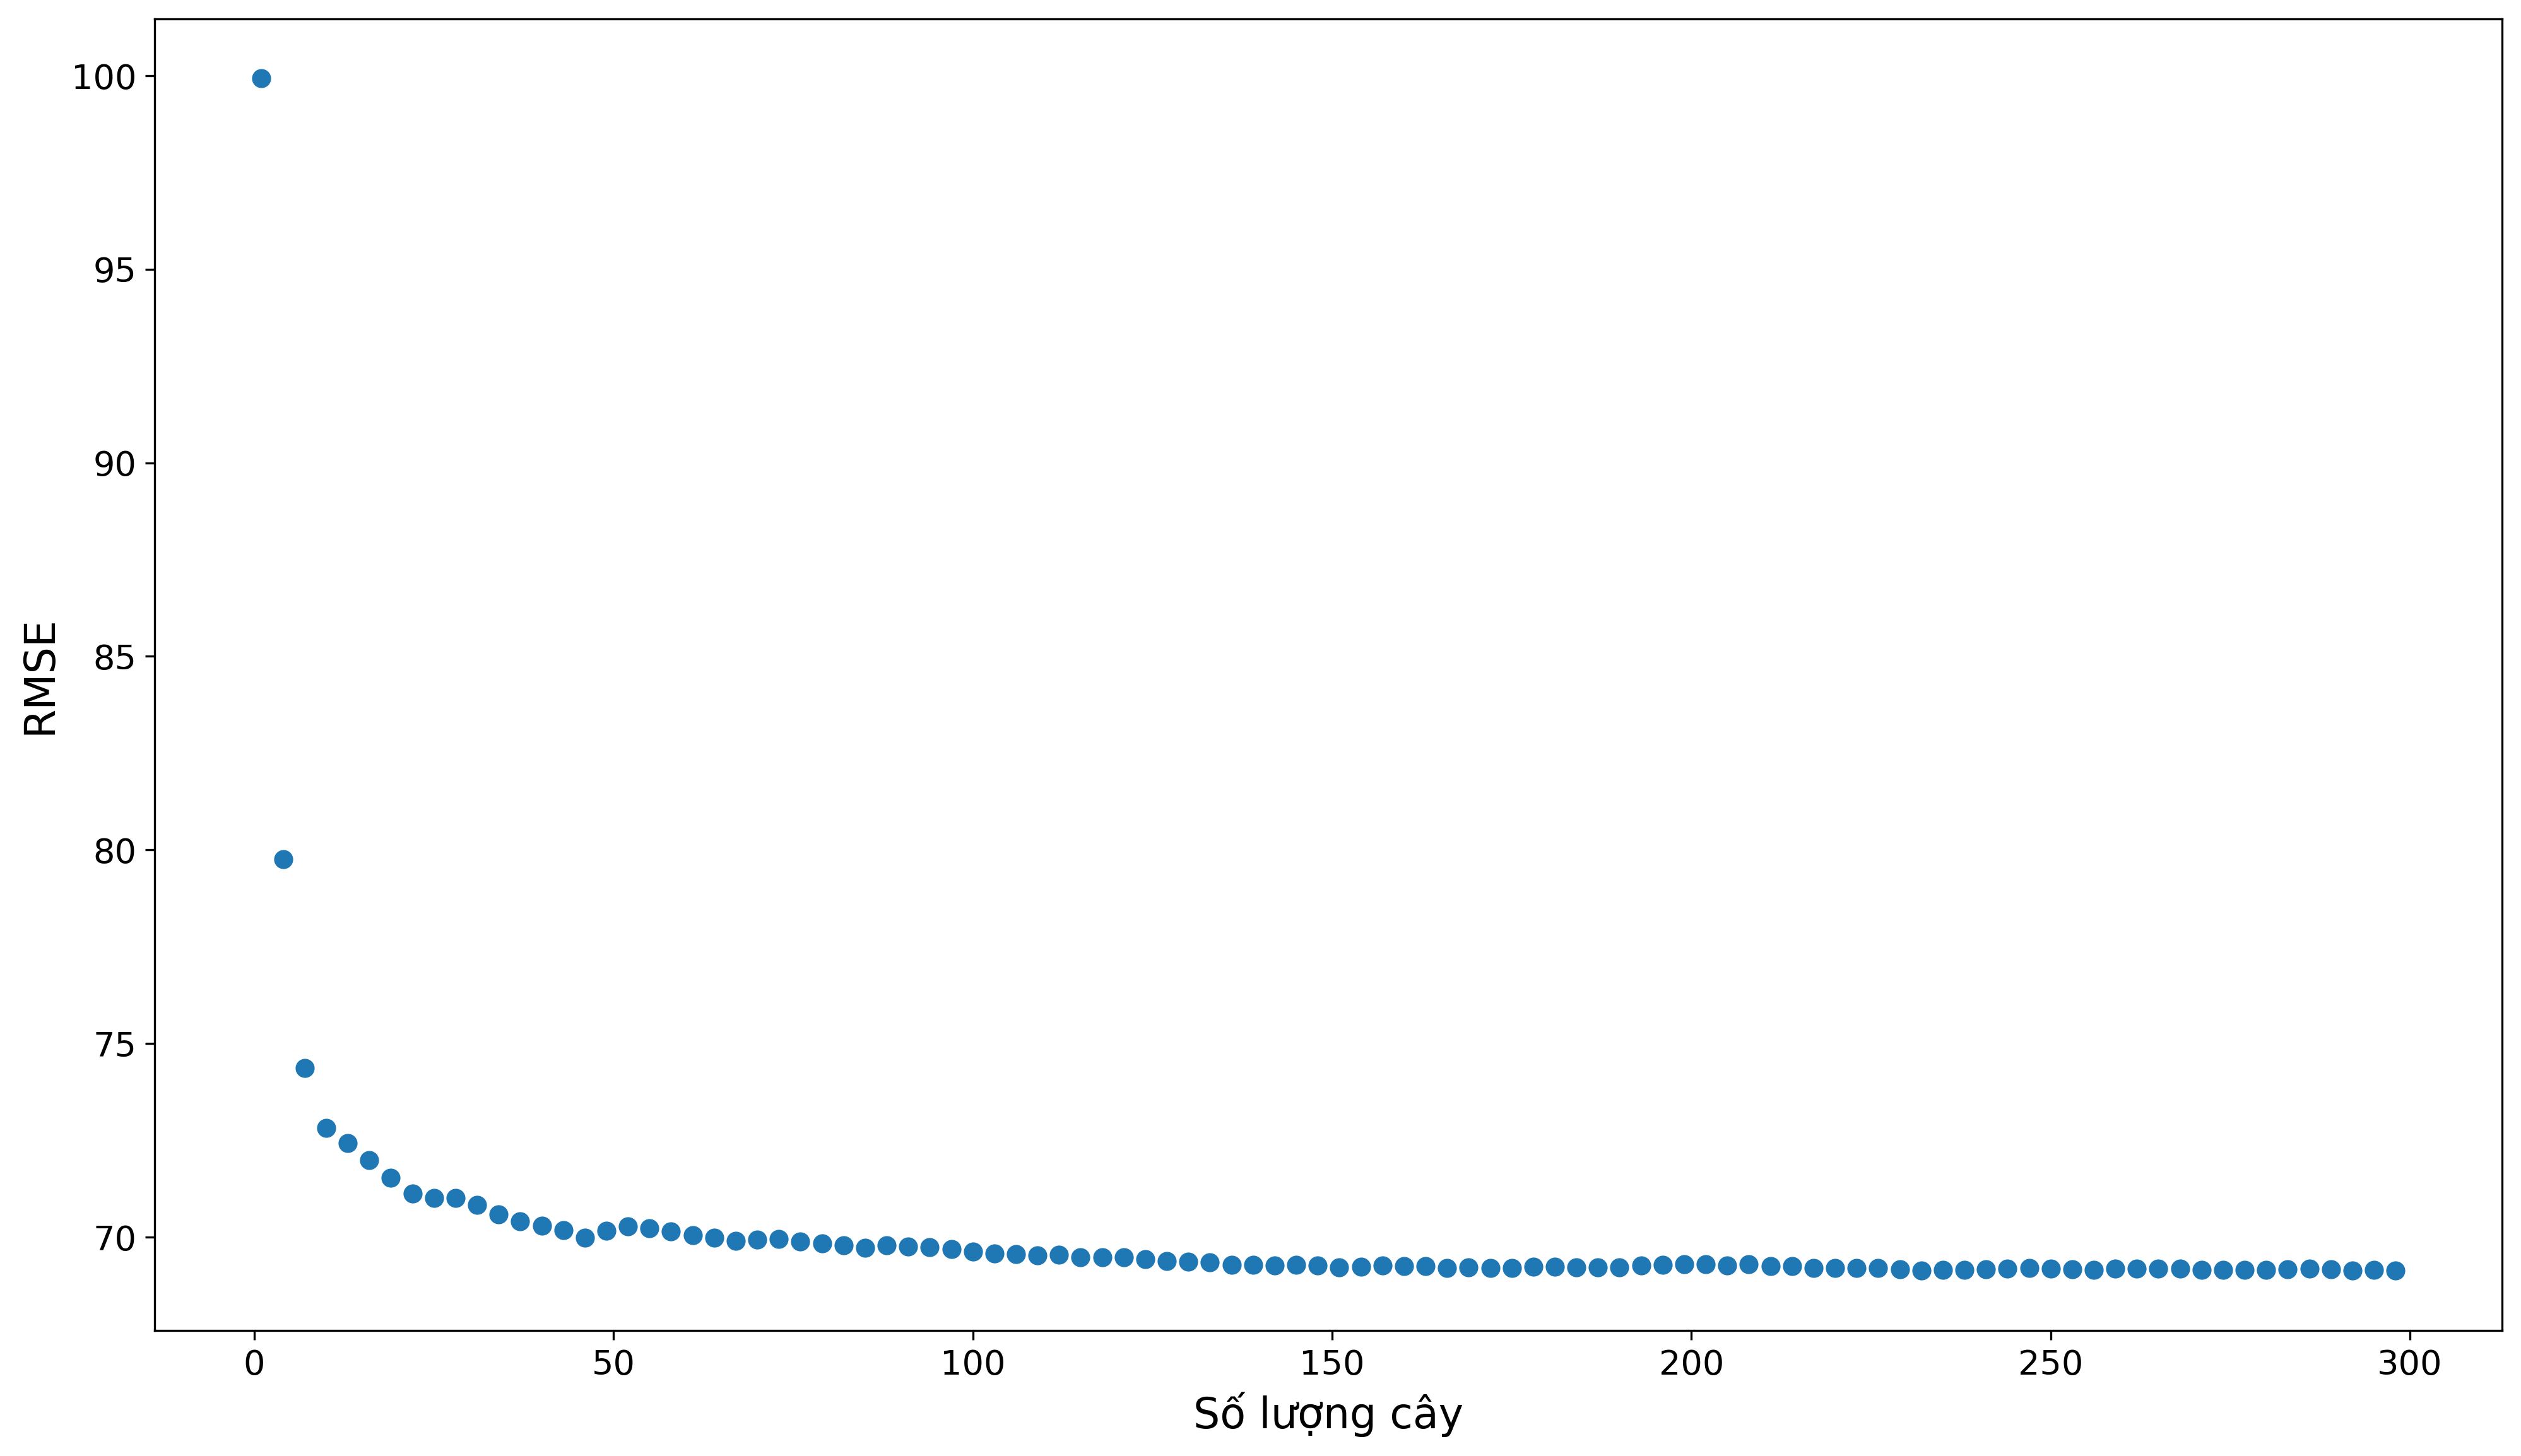
\includegraphics[width=\linewidth]{images/RF_bruteforce.png}
    \caption{Tìm số lượng cây tối ưu cho Random Forest}
\end{figure}

\subsubsection{Gradient Boosting Machine}
Gradient Boosting Machine là một mô hình dựa trên dự đoán của nhiều Decision Trees tuần tự, để tối ưu hóa mô hình, cần xác định số lượng Decision Tree của mô hình. Theo kết quả từ Hình 12, RSME của mô hình ổn định sau khoảng 1200 cây.
\begin{figure}[H]
    \centering
    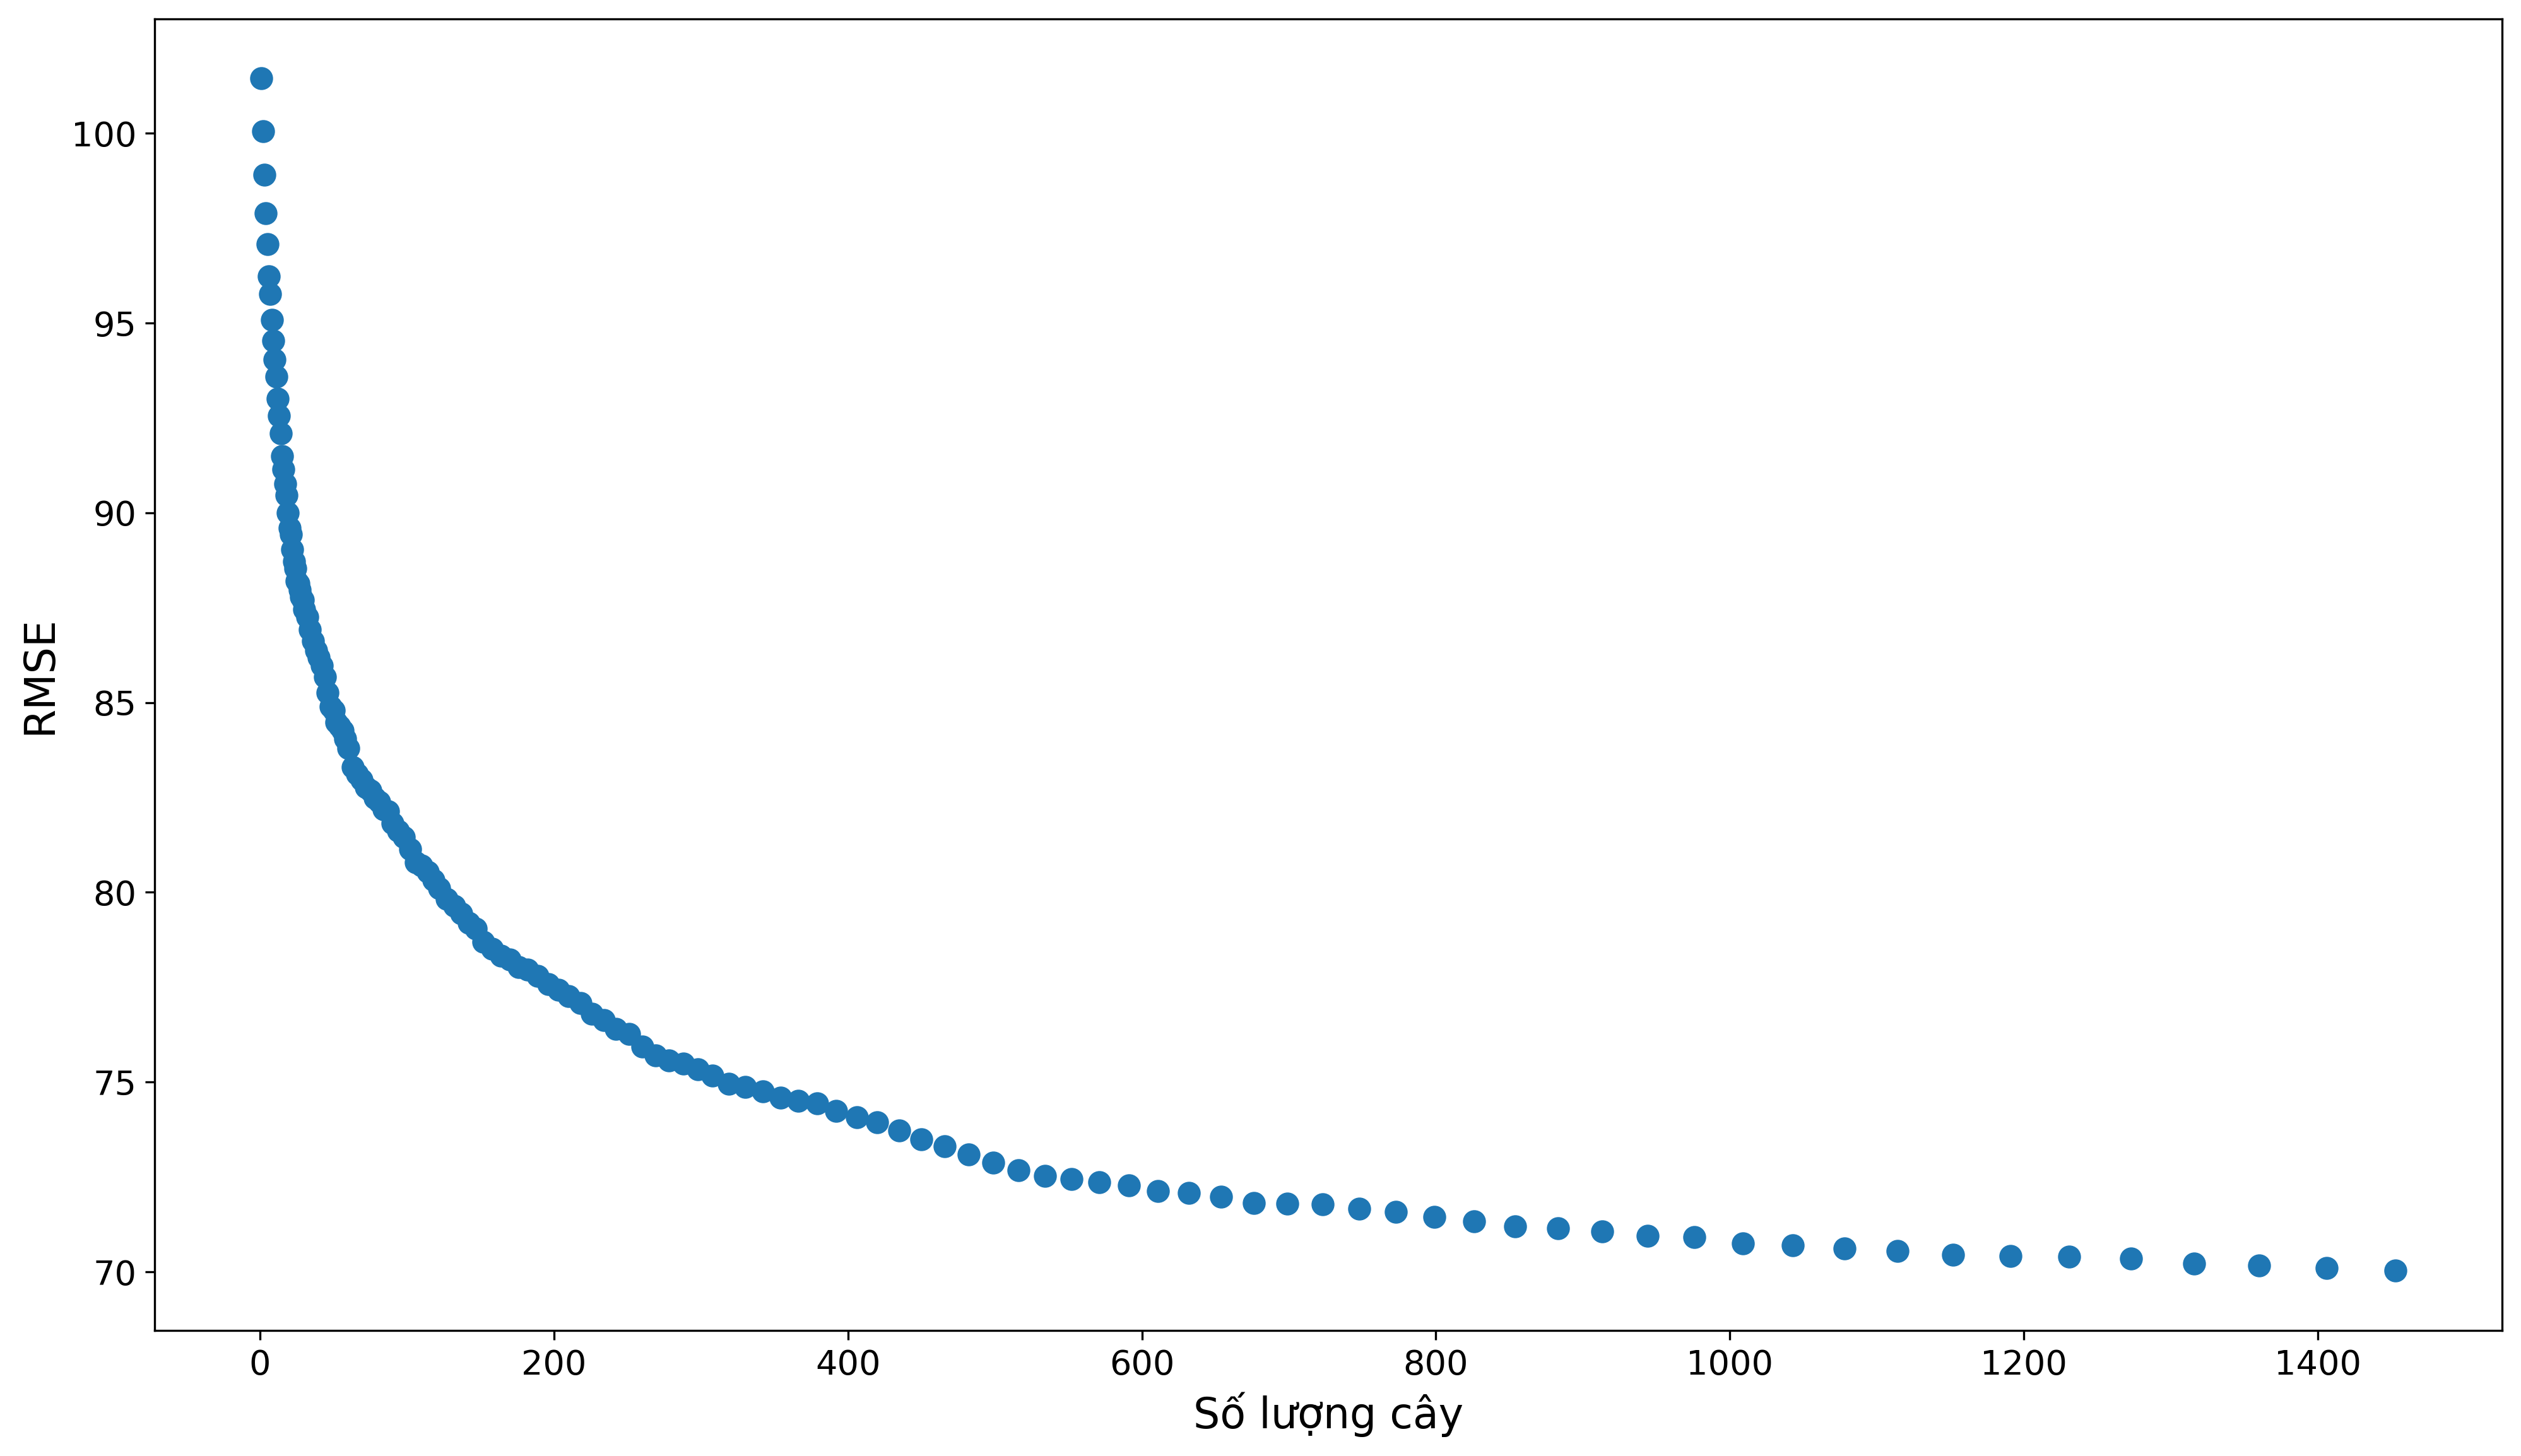
\includegraphics[width=\linewidth]{images/GBM_bruteforce.png}
    \caption{Tìm số lượng cây tối ưu cho Gradient Boosting Machine}
\end{figure}

\subsection{Đánh giá mô hình}
\subsubsection{Đánh giá mô hình hồi quy}
Hiệu suất của các mô hình được đánh giá trên tập kiểm tra thông qua chỉ số RMSE (Root Mean Squared Error), đo lường sai số bình phương trung bình giữa giá trị thực và giá trị dự đoán:
\[\text{RMSE} = \sqrt{\frac{1}{n}\sum_{i=1}^{n}{(y_i - \hat{y_i})^2}}\]

\newpage
\subsubsection{Nhận xét kết quả thực nghiệm}
Sau quá trình huấn luyện, mỗi mô hình tạo ra 30 kết quả từ việc kiểm định chéo 10-fold với 3 lần lại lại. Hình dưới đây thể hiện RMSE của từng mô hình cùng với khoảng tin cậy.
\begin{figure}[H]
    \centering
    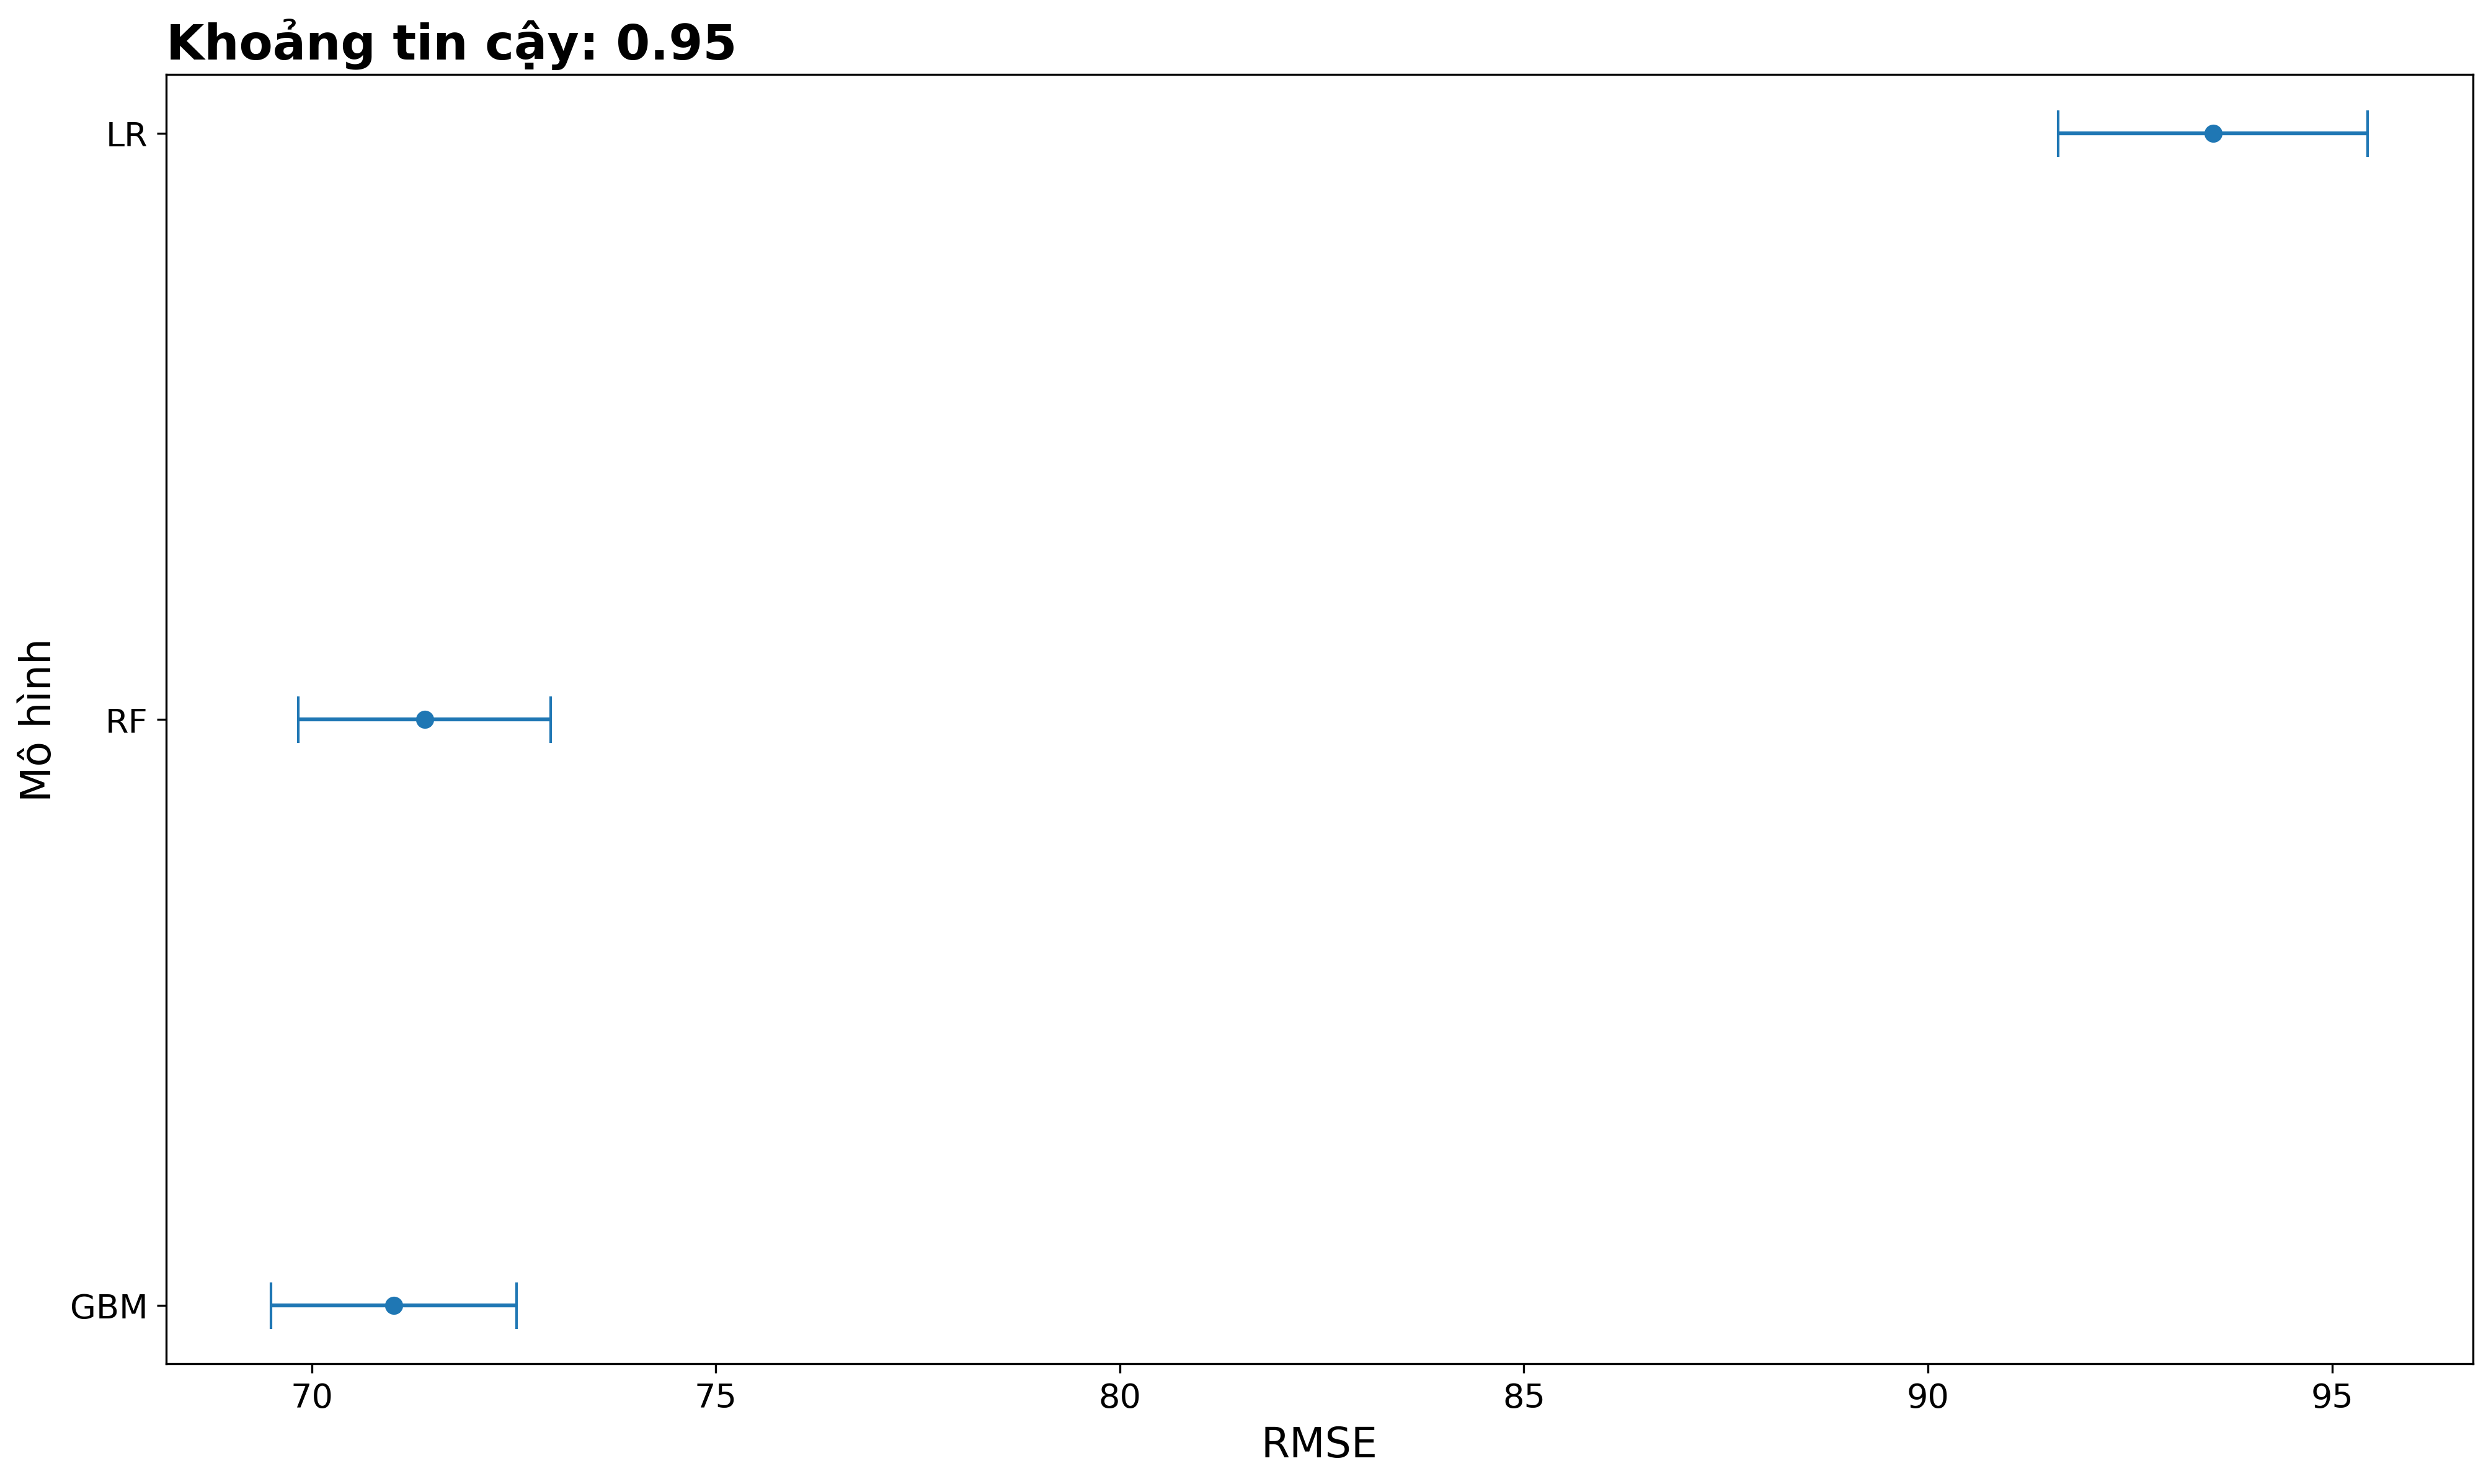
\includegraphics[width=\linewidth]{images/RMSE.png}
    \caption{So sánh RMSE của tất cả mô hình}
\end{figure}

Chúng ta có thể quan sát thấy Random Forest và Gradient Boosting Machine có hiệu suất vượt trội (RMSE thấp nhất) và tương đương nhau. Multiple Linear Regression có hiệu suất thấp nhất do không nắm bắt được mối quan hệ phi tuyến trong dữ liệu.

Bảng dưới đây cung cấp chi tiết hiệu suất của các mô hình trên tập huấn luyện và tập kiểm tra. RMSE trên tập kiểm tra nằm trong khoảng dự đoán của phần kiểm định chéo lặp lại, như trong hình trên, chứng tỏ độ tin cậy của kết quả.
\begin{table}[H]
    \centering
    \begin{tabularx}{\textwidth}{X|c|c}
         \textbf{Mô hình} &  RMSE (tập huấn luyện) & RMSE (tập kiểm tra)\\ \hline
         Multiple Linear Regression & 93.528 & 94.422\\ \hline
         Random Forest              & 71.397 & 69.131   \\ \hline
         Gradient Boosting Machine  & 71.014 & 70.43   \\
    \end{tabularx}
    \caption{Chỉ số RMSE trên tập huấn luyện và kiểm tra của 3 mô hình}
\end{table}

\newpage
Hình dưới đây thể hiện mức độ quan trọng tương đối của các biến trong các mô hình
\begin{figure}[H]
    \centering
    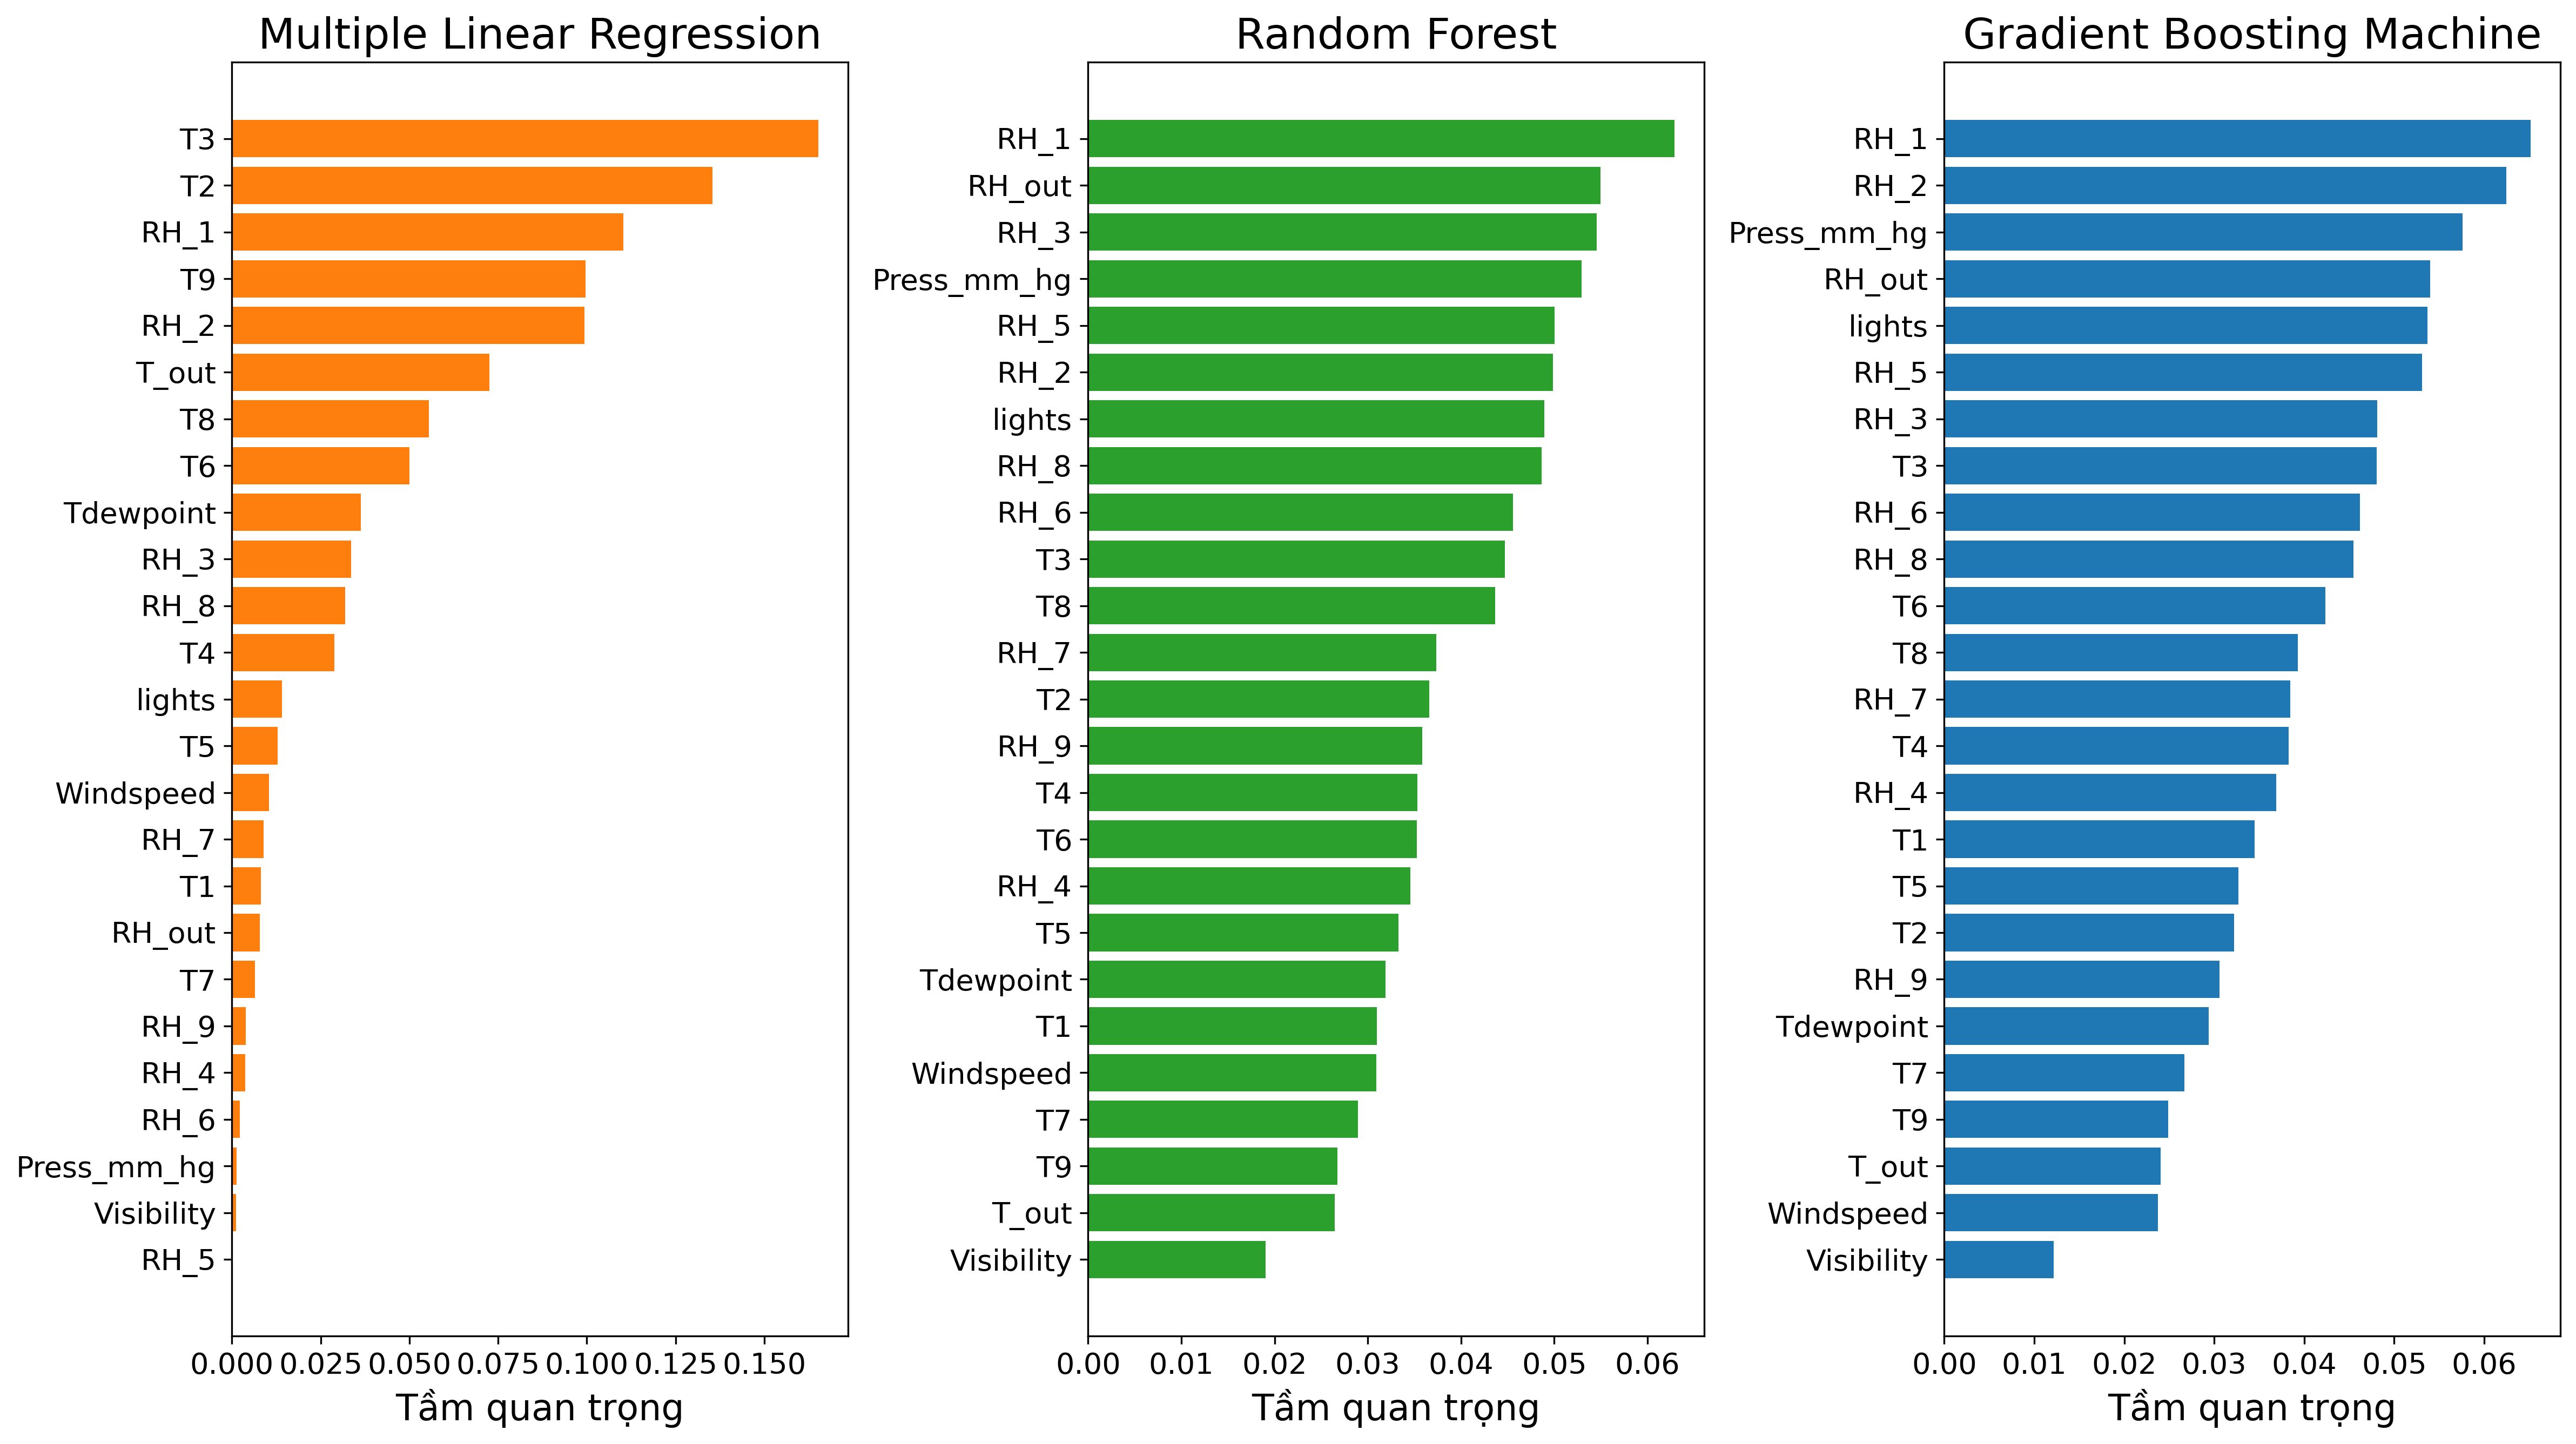
\includegraphics[width=\linewidth]{images/important.png}
    \caption{Mức độ quan trọng của các biến trong từng mô hình}
\end{figure}

Dựa trên chỉ số đánh giá RMSE, Random Forest và Gradient Boosting Machine là hai mô hình có hiệu suất tốt nhất với RMSE thấp, đồng thời thể hiện độ ổn định cao trong quá trình kiểm định chéo. Trong khi Multiple Linear Regression có hiệu suất kém nhất do không phù hợp với đặc điểm phi tuyến của dữ liệu. Mặc dù Random Forest và Gradient Boosting Machine có RMSE gần tường đương nhau, nhung Random Forest có RMSE trên tập kiểm tra là thấp nhất nên sẽ được sử dụng làm mô hình dự đoán trên ứng dụng web.